\chapter{Supporting Materials for Image Completion via Inference in Deep Generative Models}

\section{Notation}
We provide \cref{tab:cigcvae-notation} for reference as a concise list of definitions
for each symbol used in our discussion of hierarchical VAEs. More thorough explanations are provided where symbols are
introduced in the text

\begin{table*}
  \caption{Definitions for symbols used.}
  \label{tab:cigcvae-notation}
  \centering
  \begin{tabular}{rp{11cm}}
    \toprule
    Symbol    & Definition   \\
    \midrule
    $\z{}$                                   & VAE's latent variables. \\
    $\I{}$                                & Data we learn a generative model of. \\
    $\partI{}$                            & Data on which our generative model is conditioned. \\
    $\tildeI{}$                           & The part of $\I{}$ which the conditional VAE models, defined as all pixels not in $\partI{}$ for image completion, or simply $\tildeI := \I{}$ for other conditional generation tasks. \\
    $\theta$                              & Parameters for VAE's prior and decoder. \\
    $\phi$                                & Parameters for VAE's encoder. \\
    $\pdata{}(\I{}, \partI{})$            & Distribution from which we assume training/test instances are i.i.d.~samples. \\
    $\pmodel{}(\z{})$                        & Learned prior of VAE. Implicitly parameterised by $\theta$ when not otherwise specified. \\
    $\pmodel{}(\I{}|\z{})$                   & Distribution output by VAE's decoder given $\z{}$. Implicitly parameterised by $\theta$ when not otherwise specified. \\
    $q(\z{}|\I{})$                           & Distribution output by VAE's encoder given $\I{}$. Implicitly parameterised by $\phi$ when not otherwise specified. \\
    $\pmodel{}(\z{}, \I{}, \partI{})$        & Joint distribution defined as $\pmodel{}(\z{})\pmodel{}(\I{}|\z{})\pdata{}(\partI{}|\I{})$. \\
    $r(\z{},\I{}, \partI{})$                 & Joint distribution defined as $\pdata{}(\I{}, \partI{})q(\z{}|\I{})$. \\
    $\partphi$                            & Partial encoder parameters. \\
    $\partq{}(\z{}|\partI{})$                 & Distribution output by partial encoder. Implicitly parameterised by $\partphi$. \\
    $\pcomp{}(\I{}|\partI{})$             & Distribution over from which images are sampled given a conditioning input. Defined as $\int \pmodel{}(\I{}|\z{})\partq{}(\z{}|\partI{}) \mathrm{d}\z{}$. \\
    $\unp{}(\z{}, \I{}, \partI{})$           & Distribution with parameters $\optimal{\theta}$ and $\optimal{\phi}$ that are optimal as defined in \cref{proof:joint-training}. Defined equivalently as $\pmodel{}(\z{}, \I{}, \partI{}; \optimal{\theta})$ or $\pdata{}(\I{}, \partI{}) q(\z{}|\I{}; \optimal{\phi})$.  \\
    \midrule
    \multicolumn{2}{l}{Symbols for Bayesian optimal experimental design:} \\
    $\coord{}_t$                                 & The location scanned at time $t$. \\
    $v$                                   & Variable we wish to infer. \\
    $\partI{}_{\coord{}_1,\ldots,\coord{}_t}$             & Image in which all pixel values are missing except for those observed by scans at locations $\coord{}_1,\ldots,\coord{}_t$. \\
    $f_{\coord{}_1,\ldots,\coord{}_t}$                    & Function mapping from an image $\I{}$ to $\partI{}_{\coord{}_1,\ldots,\coord{}_t}$. \\
    $g(v|\partI{})$                       & Classification distribution for $v$ given partially observed image $\partI{}$. \\
    \bottomrule
  \end{tabular}
  \vspace{-1em}
\end{table*}


\section{Expanded derivations}
\subsection{Expanded derivation of \cref{eq:elbo-kl-joints}}
Here we expand on the steps to show that the expectation of the ELBO in
\cref{eq:eelbo} is equivalent to the lower bound on the negative entropy of
$\pdata{}(\I{})$ in \cref{eq:elbo-kl-joints}.
\begin{align}
  \EX_{\pdata{}(\I{})} \left[ \text{ELBO}(\theta, \phi, \I{}) \right] &= \EX_{\pdata(\I{})} \EX_{q(\z{}|\I{}; \phi)} \left[ \log\frac{\pmodel{}(\z{}; \theta)\pmodel{}(\I{}|\z{}; \theta)}{q(\z{}|\I{}; \phi)} \right] \label{eq:eelbo-repeat}\\
                                                                      &= \EX_{\pdata(\I{})q(\z{}|\I{}; \phi)} \left[ \log\frac{\pmodel{}(\z{}, \I{}; \theta)}{q(\z{}|\I{}; \phi)} \right] \\
                                                                      &= \EX_{\pdata(\I{})q(\z{}|\I{}; \phi)} \left[ \log\pdata{}(\I{}) + \log\frac{\pmodel{}(\z{}, \I{}; \theta)}{\pdata{}(\I{})q(\z{}|\I{}; \phi)} \right] \\
                                                                      &= \EX_{\pdata(\I{})} \left[ \log\pdata(\I{}) \right] + \EX_{\pdata(\I{})q(\z{}|\I{}; \phi)} \left[ \log\frac{\pmodel{}(\z{}, \I{}; \theta)}{\pdata{}(\I{})q(\z{}|\I{}; \phi)} \right] \\
                                                                      &= -\mathcal{H}\left[ \pdata(\I) \right] - \kl[\big] { \pdata{}(\I{})q(\z{}|\I{}; \phi) }{ \pmodel{}(\z{}, \I; \theta) } \label{eq:elbo-kl-joints-repeat}
\end{align}
as written in \cref{eq:elbo-kl-joints}.

\subsection{Expanded derivation of \cref{eq:forward-elbo}} \label{supp:cigcvae-forward-elbo-bound-deriv}
Here we prove \cref{eq:forward-elbo}, which states that IPA's training
objective is a lower bound on $\EX_{\pdata{}(\I{}, \partI{})} \left[ \log
  \pcomp{}(\tildeI{}|\partI{}) \right]$.
\begin{align}
  \mathcal{O}_\mathrm{for}(\theta, \phi, \partphi{}) &= \EX_{\pdata{}(\I{}, \partI{})} \EX_{q(\z{}|\I{})} \left[ \log \frac{\pmodel{}(\tildeI{}|\z{})\partq{}(\z{}|\partI{})}{q(\z{}|\I{})} \right] \\
                                                   &\leq \EX_{\pdata{}(\I{}, \partI{})} \left[ \log \EX_{q(\z{}|\I{})} \left[ \frac{\pmodel{}(\tildeI{}|\z{})\partq{}(\z{}|\partI{})}{q(\z{}|\I{})} \right]  \right] \\
                                                   &= \EX_{\pdata{}(\I{}, \partI{})} \left[ \log \EX_{\partq{}(\z{}|\partI{})} \left[ \pmodel{}(\tildeI{}|\z{}) \right]  \right] \\
                                                   &= \EX_{\pdata{}(\I{}, \partI{})} \left[ \log \pcomp{}(\tildeI{}|\partI{}) \right],
\end{align}
where the final step follows from the definition of $\pcomp{}$ in
\cref{eq:marginal-image-posterior}.


% \section{Proofs} \label{supp:cigcvae-proofs}

\section{Proof and discussion of Theorem~\ref{theorem:forward-kl}} \label{proof:forward-kl}
\subsection{Proof}
\textbf{Statement.}
\textit{
  For any set $\Partphi$ of
  permissible values of $\partphi{}$, and for any $\theta\in\Theta$ and
  $\phi\in\Phi$,
  \begin{equation}
    \argmax_{\partphi{} \in \Partphi} \mathcal{O}_\mathrm{for}(\theta, \phi, \partphi{}) = \argmin_{\partphi{} \in \Partphi} \EX_{\pdata{}(\partI{})} \left[ \kl[\big]{ r(\z{}|\partI{}) }{ \partq{}(\z{}|\partI{}) } \right]. \tag{\ref{eq:forward-theorem}}
  \end{equation}
}

\textbf{Proof.} We can decompose $\mathcal{O}_\mathrm{for}$ as follows.
Starting by multiplying both sides of the fraction by the intractable
conditional distribution $r(\z{}|\partI{})$,
\begin{align}
  \mathcal{O}_\mathrm{for}(\theta, \phi, \partphi{}) &= \EX_{r(\z{},\I{},\partI{})} \left[ \log \frac{\pmodel{}(\tildeI{}|\z{})\partq{}(\z{}|\partI{})r(\z{}|\partI{})}{q(\z{}|\I{})r(\z{}|\partI{})} \right]\\
                                                   &= \EX_{r(\z{},\I{},\partI{})} \left[ \log \frac{\pmodel{}(\tildeI{}|\z{})r(\z{}|\partI{})}{q(\z{}|\I{})} \right] - \EX_{r(\z{},\partI{})} \left[ \log\frac{r(\z{}|\partI{})}{\partq{}(\z{}|\partI{})} \right] \\
                                                   &= C(\theta, \phi) - \EX_{\pdata{}(\partI{})} \left[ \kl[\big]{ r(\z{}|\partI{}) }{ \partq{}(\z{}|\partI{}) } \right]   \label{eq:constant-and-forward-kl}
\end{align}
where $C(\theta, \phi)$ is a grouping of terms which do not depend on the
partial encoder's parameters $\partphi{}$. Any values of $\partphi{}$ which
maximise $\mathcal{O}_\mathrm{for}(\theta, \phi, \partphi{})$ will therefore also
minimise $\EX_{\pdata{}(\partI{})} \left[ \kl[\big]{ r(\z{}|\partI{}) }{
    \partq{}(\z{}|\partI{}) } \right]$ for the same values of $\theta$ and $\phi$,
which proves the theorem.

\subsection{Bound on $\tildeI{}$-space divergence}
The mass-covering KL divergence in \Cref{theorem:forward-kl} indicates that
samples $\z{}\sim \partq{}(\cdot|\partI{})$ will be diverse (when $r(\z{}|\partI{})$ is
diverse/uncertain). One would expect that samples of $\tildeI{}$ conditioned on these
diverse samples of $\z{}$ will also be diverse. Here we make a more formal argument
by showing that minimising $\mathcal{O}_\mathrm{for}$ corresponds to miminising
an upper-bound on an expected mass-covering KL divergence in $\tildeI{}$-space.
Starting from the result in \cref{supp:cigcvae-forward-elbo-bound-deriv},
\begin{align}
  \mathcal{O}_\mathrm{for}(\theta, \phi, \partphi{}) &\leq \EX_{\pdata{}(\I{},\partI{})} \left[ \log \pcomp{}(\tildeI{}|\partI{}) \right] \\
                                                     &= \EX_{\pdata{}(\I{},\partI{})} \left[ \log \pdata{}(\tildeI{}|\partI{}) \right] - \EX_{\pdata{}(\partI{})}\left[ \kl{\pdata{}(\tildeI{}|\partI{})}{\pcomp{}(\tildeI{}|\partI{})} \right].
\end{align}
Rearranging this gives
\begin{align}
  \EX_{\pdata{}(\partI{})}\left[ \kl{\pdata{}(\tildeI{}|\partI{})}{\pcomp{}(\tildeI{}|\partI{})} \right]  \leq \EX_{\pdata{}(\I{},\partI{})} \left[ \log \pdata{}(\tildeI{}|\partI{}) \right] - \mathcal{O}_\mathrm{for}(\theta, \phi, \partphi{}).
\end{align}
Maximising $\mathcal{O}_\mathrm{for}$ therefore minimises an upper-bound on an
expected mass-covering KL divergence in $\tildeI{}$-space, providing a further suggestion that
$\tildeI{}\sim\pcomp{}(\cdot|\partI{})$ will be diverse.


\section{Proof and discussion of Theorem~\ref{theorem:joint-training}}  \label{proof:joint-training}
\subsection{Proof}

\textbf{Statement.} \textit{Assume that we have a sufficiently expressive
  encoder and decoder that there exist parameters $\optimal{\theta}\in\Theta$
  and $\optimal{\phi}\in\Phi$ which make the unconditional VAE objective
  (\cref{eq:eelbo}) equal to its upper bound of $-\mathcal{H}\left[ \pdata(\I)
  \right]$. Assume also that the mutual information ${\mutinf{} :=
  \EX_{\pmodel{}(\tildeI{}, \partI{}, \z{}; \theta^*)} \left[ \log
    \frac{\pmodel{}(\tildeI{},\partI{}|\z{}; \theta^*) }{ \pmodel{}(\tildeI{}|\z{};
      \theta^*)\pmodel{}(\partI{}|\z{}; \theta^*) } \right] =
  \EX_{\pmodel{}(\tildeI{}, \partI{}, \z{}; \theta^*)} \left[ \log
    \frac{\pmodel{}(\tildeI{}|\z{}, \partI{}; \theta^*) }{ \pmodel{}(\tildeI{}|\z{};
      \theta^*) } \right]}$ is zero (meaning that $\tildeI{}$ and $\partI{}$ are
  conditionally independent given $\z{}$) and $\tildeI{}$ is defined such that there
  exists a mapping from $(\tildeI{},\partI{})$ to $\I{}$. Then, given a
  sufficiently expressive partial encoder $\partq{}(\z{}|\partI{}; \partphi)$, }
\begin{equation} \tag{\ref{eq:joint-training}}
  \max_{\partphi{}} \mathcal{O}_\mathrm{for}(\optimal{\theta}, \optimal{\phi}, \partphi{}) = \max_{\theta, \phi, \partphi{}} \mathcal{O}_\mathrm{for}(\theta, \phi, \partphi{}).
\end{equation}

\textbf{Proof.} We have used, and will continue to use, $\pmodel{}(\cdot)$ and
$q(\cdot)$ to refer to joint distributions parameterised by $\theta$ and $\phi$
respectively. Since $\optimal{\theta}$ and $\optimal{\phi}$ are defined as the
maximisers of the unconditional ELBO in \cref{eq:elbo-kl-joints}, and given our
assumption of sufficient expressivity, we have $\pmodel{}(\z{}, \I{};
\optimal{\theta}) = \pdata{}(\I{}) q(\z{}|\I{}; \optimal{\phi})$. We can therefore
introduce notation for the equal joint distributions: $\optimal{p}(\z{}, \I{},
\partI{}) = \pmodel{}(\z{}, \I{}, \partI{}; \optimal{\theta}) = \pdata{}(\I{},
\partI{}) q(\z{}|\I{}; \optimal{\phi})$. We note that we can also write the joint
distribution $\optimal{p}(\z{}, \I{}, \tildeI{}, \partI{}) = \pdata{}(\I{},
\partI{}) q(\z{}|\I{}; \optimal{\phi})p(\tildeI{}|\I{},\partI{})$, where
$p(\tildeI{}|\I{},\partI{})=\delta_{g(\I{},\partI{})}(\tildeI{})$ is the Dirac
distribution mapping $\I{}$ and $\partI{}$ deterministically to
$\tildeI{}=g(\I{},\partI{})$.
%
Recalling that we define $\tildeI{}$ as either equal to $\I{}$ or as the
dimensions of $\I{}$ not observed in $\partI{}$, such a deterministic $g$ will
always exist.

% We note that defining this
% joint distribution also implicitly defines $\optimal{p}(\z{}, \tildeI{}, \partI{})$
% as a marginal (over any elements of $\I{}$ not in $\tildeI{}$).

We consider the decomposition of $\mathcal{O}_\mathrm{for}$ shown in
\cref{eq:constant-and-forward-kl} and remind the reader that, given a
sufficiently expressive partial encoder, the maximisation over $\partphi$ will
always make the KL divergence zero. That is,
\begin{equation}
  \max_{\partphi{}} \mathcal{O}_\mathrm{for}(\theta, \phi, \partphi{}) = C(\theta, \phi) = \EX_{r(\z{},\I{},\partI{})} \left[ \log \frac{\pmodel{}(\tildeI{}|\z{})r(\z{}|\partI{})}{q(\z{}|\I{})} \right] \label{eq:forward-max-phi}
\end{equation}
for any $\theta$ and $\phi$. Using $\optimal{\theta}$ and $\optimal{\phi}$, and
therefore using $\unp{}$ in place of $\pmodel{}$, $r$ and $q$, we can expand the
left-hand side of \cref{eq:joint-training}.
\begin{align}
  \max_{\partphi{}} \mathcal{O}_\mathrm{for}(\optimal{\theta}, \optimal{\phi}, \partphi{}) &= \EX_{\unp{}(\z{},\I{},\partI{})} \left[ \log \frac{\unp{}(\tildeI{}|\z{})\unp{}(\z{}|\partI{})}{\unp(\z{}|\I{})} \right] \\
                                                                                           &= \EX_{\unp{}(\z{},\I{},\partI{})} \left[ \log \frac{\unp{}(\tildeI{}|\z{},\partI{})\unp{}(\z{}|\partI{})}{\unp(\z{}|\I{})} \right] - \EX_{\unp{}(\z{},\tildeI{},\partI{})} \left[ \log\frac{\unp{}(\tildeI{}|\z{},\partI{})}{\unp{}(\tildeI{}|\z{})} \right] \\
                                                                                           &= \EX_{\unp{}(\z{},\I{},\partI{})} \left[ \log \frac{\unp{}(\tildeI{}|\z{},\partI{})\unp{}(\z{}|\partI{})}{\unp(\z{}|\I{})} \right] - \mutinf{}\\
                                                                                           &= \EX_{\unp{}(\z{},\I{},\partI{})} \left[ \log \frac{\unp{}(\z{},\tildeI{}|\partI{})}{\unp(\z{}|\I{})} \right] - \mutinf{}\\
                                                                                           &= \EX_{\unp{}(\z{},\I{},\partI{})} \left[ \log \frac{\unp{}(\z{}|\tildeI{},\partI{})\unp{}(\tildeI{}|\partI{})}{\unp(\z{}|\I{})} \right] - \mutinf{}. \label{eq:pre-mapping}
\end{align}
% Here, we note that we can make the factorisation $\optimal{p}(\z{}, \I{},
% \tildeI{}, \partI{}) = \pdata{}(\I{}, \partI{}) q(\z{}|\I{};
% \optimal{\phi})\delta(\tildeI{}|\I{},\partI{})$, where
% $\delta(\tildeI{}|\I{},\partI{})$ is the Dirac distribution mapping $\I{}$ and
% $\partI{}$ deterministically to $\tildeI{}$, which we have previously made
% implicit. 
The factorisation $\optimal{p}(\z{}, \I{}, \tildeI{}, \partI{}) = \pdata{}(\I{},
\partI{}) q(\z{}|\I{}; \optimal{\phi})\delta(\tildeI{}|\I{},\partI{})$ implies that
we can express $\unp{}(\z{}|\tildeI{},\partI{})$ with a marginalisation:
$\unp{}(\z{}|\tildeI{},\partI{})=\int \unp{}(\z{}|\I{})
\unp{}(\I{}|\tildeI{},\partI{}) \mathrm{d}\I{}$. Since we have assumed that
there is a deterministic function $f$ mapping $(\tildeI{},\partI{})$ to $\I{}$,
$\unp{}(\I{}|\tildeI{},\partI{})$ is a Dirac distribution and the
marginalisation becomes $\unp{}(\z{}|\tildeI{},\partI{}) = \int \unp{}(\z{}|\I{})
\delta(\I{}|\tildeI{},\partI{}) \mathrm{d}\I{} =
\unp{}(\z{}|\I{}=f(\tildeI{},\partI{}))$. We therefore proceed, rewriting
$\unp{}(\z{}|\tildeI{},\partI{})$ as $\unp{}(\z{}|\I{})$:
\begin{align}
  \max_{\partphi{}} \mathcal{O}_\mathrm{for}(\optimal{\theta}, \optimal{\phi}, \partphi{}) &= \EX_{\unp{}(\z{},\I{},\partI{})} \left[ \log \frac{\unp{}(\z{}|\I{})\unp{}(\tildeI{}|\partI{})}{\unp(\z{}|\I{})} \right] - \mutinf{} \label{eq:post-mapping}\\
                                                                                           &= \EX_{\unp{}(\I{},\partI{})} \left[ \log \unp{} (\tildeI{}|\partI{}) \right] - \mutinf{}\\
                                                                                           &= \EX_{\pdata{}(\I{},\partI{})} \left[ \log \pdata{} (\tildeI{}|\partI{}) \right] - \mutinf{}. \label{eq:max-partphi-bound}
\end{align}
Now that we have this expansion of the left-hand side of
\cref{eq:joint-training}, we can derive a related upper-bound on the right-hand
side as follows. For any $\theta$, any $\phi$, and any $\partphi$, we have
from \cref{supp:cigcvae-forward-elbo-bound-deriv}:
\begin{align}
  \mathcal{O}_\mathrm{for}(\theta, \phi, \partphi{}) &\leq \EX_{\pdata{}(\I{},\partI{})} \left[ \log \pcomp{}(\tildeI{}|\partI{}) \right] \\
                                                     &= \EX_{\pdata{}(\I{},\partI{})} \left[ \log \pdata{}(\tildeI{}|\partI{}) \right] - \EX_{\pdata{}(\partI{})}\left[ \kl{\pdata{}(\tildeI{}|\partI{})}{\pcomp{}(\tildeI{}|\partI{})} \right] \\
                                                     &\leq \EX_{\pdata{}(\I{},\partI{})} \left[ \log \pdata{}(\tildeI{}|\partI{}) \right].
\end{align}
This bound must also hold for the maximum over $\theta$, $\phi$, and
$\partphi$, and so is an upper-bound on the right-hand side of \cref{eq:joint-training}:
\begin{align}
  \max_{\theta, \phi, \partphi{}} \mathcal{O}_\mathrm{for}(\theta, \phi, \partphi{}) &\leq \EX_{\pdata{}(\I{},\partI{})} \left[ \log \pdata{}(\tildeI{}|\partI{}) \right]. \label{eq:max-all-bound}
\end{align}

By relating \cref{eq:max-partphi-bound} and \cref{eq:max-all-bound}, we have:
\begin{align}
  \max_{\theta, \phi, \partphi{}} \mathcal{O}_\mathrm{for}(\theta, \phi, \partphi{}) &\leq  \max_{\partphi{}} \mathcal{O}_\mathrm{for}(\optimal{\theta}, \optimal{\phi}, \partphi{}) + \mutinf{}. \label{eq:bound-1}
\end{align}
We then point out that we can also obtain an inequality in the other direction: since
the right-hand side of \cref{eq:joint-training} is a maximisation of the left-hand side over $\theta$ and
$\phi$, it must be greater than or equal to the left-hand side:
\begin{align}
  \max_{\partphi{}} \mathcal{O}_\mathrm{for}(\optimal{\theta}, \optimal{\phi}, \partphi{}) &\leq  \max_{\theta, \phi, \partphi{}} \mathcal{O}_\mathrm{for}(\theta, \phi, \partphi{})  . \label{eq:bound-2}
\end{align}
Combining \cref{eq:bound-1} and \cref{eq:bound-2}, we have:
\begin{align}
  0 \leq \max_{\theta, \phi, \partphi{}} \mathcal{O}_\mathrm{for}(\theta, \phi, \partphi{}) - \max_{\partphi{}} \mathcal{O}_\mathrm{for}(\optimal{\theta}, \optimal{\phi}, \partphi{}) \leq \mutinf{}. \label{eq:two-bounds}
\end{align}
We now have bounds in both directions on the difference between the right- and
left-hand sides. To conclude the proof, we repeat the assumption that
$\mutinf{}=0$. The upper- and lower- bounds of \cref{eq:two-bounds} are
therefore both zero, so we have the final result that ${\max_{\partphi{}}
\mathcal{O}_\mathrm{for}(\optimal{\theta}, \optimal{\phi}, \partphi{}) =
\max_{\theta, \phi, \partphi{}} \mathcal{O}_\mathrm{for}(\theta, \phi,
\partphi{})}$.

\subsection{Discussion of the assumption that $\mutinf{}=0$}
The above proof of \cref{theorem:joint-training} relies on the assumption that
$\mutinf{} = \EX_{\unp{}(\tildeI{}, \partI{}, \z{})} \left[ \log
  \frac{\unp{}(\tildeI{}|\z{}, \partI{}) }{ \unp{}(\tildeI{}|\z{}) } \right] = 0$.
That is, under the joint distribution $p^*(\z{},\I{},\partI{})$, $\tildeI{}$ and
$\partI{}$ should be conditionally independent given $\z{}$. We now argue that this
is true for image completion, and ``close to'' satisfied \textcolor{black}{when
  $\mathbf{y}$ consists of high-level image features. This means that
  \cref{theorem:joint-training} is informative for inpainting, our
  edges-to-photos experiments and, e.g., class-conditional generation but may
  not even approximately hold for, e.g., super-resolution or image
  colourisation.}

\paragraph{Image completion}
In the VAE architecture we use, the likelihood $\pmodel{}(\I{}|\z{})$ is pixel-wise
independent. In other words, if we write $\I{}$ as a set of pixels
$\{\I{}_1,\ldots,\I{}_N\}$, we can factorise $\pmodel{}(\I{}|\z{})$ as
$\prod_{i=1}^N\pmodel{}(\I{}_i|\z{})$. This means that the conditional mutual
information between any two disjoint subsets of $\I{}$ (conditioned on $\z{}$) will
be zero. Given our definition of $\tildeI{}$ for image completion as the the set
of purely unobserved pixels, we have by construction that $\tildeI{}$ and
$\partI{}$ are disjoint. Therefore, the assumption that $\mutinf{}=0$ is
satisfied for image completion.

% In our exposition, $\I{}$ and $\partI{}$ are not disjoint (since we
% defined $\I{}$ to be the set of all image pixels including those in $\partI{}$),
% and so the conditional mutual information between them need not be zero.
% However, we could alternatively have used an objective which only optimised a
% lower-bound on the likelihood of unobserved pixels. Denoting the unobserved
% pixels $\I{}\setminus\partI{}$, this lower-bound is an alteration of that in
% \cref{eq:forward-elbo}:
% \begin{align}
%   \label{eq:forward-elbo-sub}
%   \mathcal{O}^\text{sub}_\mathrm{for}(\theta, \phi, \partphi{}) &= \EX_{\pdata{}(\I{}, \partI{})} \EX_{q(\z{}|\I{})} \left[ \log \frac{\pmodel{}(\I{}\setminus\partI{}|\z{})\partq{}(\z{}|\partI{})}{q(\z{}|\I{})} \right] &\leq \EX_{\pdata{}(\I{}, \partI{})} \left[ \log \pcomp{}(\I{}\setminus\partI{}|\partI{}) \right].
% \end{align}
% Note that training IPA with this objective is equivalent to training IPA with
% $\mathcal{O}_\mathrm{for}$. This is because both the term that has changed,
% $\pmodel(\I{}|\z{})$, and its replacement $\pmodel{}(\I{}\setminus\partI{}|\z{})$,
% are independent of $\partphi$. The gradients with respect to $\partphi$ are
% therefore exactly the same for $\mathcal{O}_\mathrm{for}$ and
% $\mathcal{O}^\text{sub}_\mathrm{for}$. Since IPA only optimises $\partphi$, it
% will therefore be identical for either objective.

% For the new objective $\mathcal{O}_\mathrm{for}$, we can derive an analogy to
% \cref{eq:two-bounds}.
% \begin{align}
%   0 \leq \max_{\theta, \phi, \partphi{}} \mathcal{O}^\text{sub}_\mathrm{for}(\theta, \phi, \partphi{}) - \max_{\partphi{}} \mathcal{O}^\text{sub}_\mathrm{for}(\optimal{\theta}, \optimal{\phi}, \partphi{}) \leq \mutinfsub{}
% \end{align}
% where $\mutinfsub := \EX_{\pmodel{}(\I{}, \partI{}, \z{}; \theta^*)} \left[\log
%   \frac{\unp{}(\I{}\setminus\partI{}|\z{}, \partI{}) }{ \unp{}(\I{}|\z{}) } \right]$.
% The derivation of this is almost identical to that of \cref{eq:two-bounds}, if
% $\mathcal{O}_\mathrm{for}$ is replaced with
% $\mathcal{O}^\text{sub}_\mathrm{for}$, and $\mutinf$ is replaced with
% $\mutinfsub$. Since $\I{}\setminus\partI{}$ and $\partI{}$ are disjoint subsets
% of image pixels, we have that $\mutinfsub{}=0$ and so the upper and lower bounds
% are the same, leading to the equality:
% \begin{align}
%   \max_{\theta, \phi, \partphi{}} \mathcal{O}^\text{sub}_\mathrm{for}(\theta, \phi, \partphi{}) = \max_{\partphi{}} \mathcal{O}^\text{sub}_\mathrm{for}(\optimal{\theta}, \optimal{\phi}, \partphi{}).
% \end{align}


\paragraph{When $\mutinf{}$ is non-zero.}
When $\mutinf{}$ is non-zero, we can still use it as an upper-bound on the
difference between the left- and right-hand side of \cref{eq:joint-training}
using \cref{eq:two-bounds}.
%
Moreover, we posit that $\mutinf{}$ will typically be small when $\partI{}$
represents high-level features (e.g.~the edges in Edges2Photos or a class label)
and we have a pixel-wise independent likelihood. This is because any high-level
structure cannot be modelled by the pixel-wise independent likelihood
$\unp{}(\tildeI{}|\z{})$ and so must be captured by $\z{}$. Intuitively, high-level
features $\partI{}$ are unlikely to be informative about any pixel-level
variations if all image structure spanning multiple pixels ($\z{}$) is already
known. This is equivalent to saying that $\mutinf{}$, the mutual information
between $\tildeI{}$ and $\partI{}$ conditioned on $\z{}$, is likely to be small.

\section{An alternative training objective}
\label{supp:cigcvae-ipa-r}
In this section, we describe an alternative objective previously used by
\citet{ma2018eddi}. We find experimentally that its performance is typically
worse than $\mathcal{O}_\mathrm{for}$, but it has the advantage of only
requiring data $\partI{} \sim \pdata{}(\cdot)$ during training, and not $\I{}$.
This may allow training in settings such as
outpainting~\citep{sabini2018painting}. The objective can be interpreted as a
lower bound on $\log \pmodel{}(\partI{})$:
\begin{align} \label{eq:reverse-obj}
  \mathcal{O}_\text{rev}(\theta, \phi, \partphi{}) &= \EX_{\pdata{}(\partI{})}\EX_{\partq{}(\z{}|\partI{})} \left[ \log\frac{\pmodel{}(\z{},\partI{})}{\partq{}(\z{}|\partI{})} \right] \leq \EX_{\pdata{}(\partI{})} \left[ \log \pmodel(\partI{}) \right].
\end{align}
Computing this objective requires a computation graph similar to that shown in
\cref{fig:cigcvae-reverse-arch}. Note one caveat with this objective is that using it
involves computing and differentiating $\pmodel{}(\z{},\partI{})$, which requires a
tractable likelihood $\pdata{}(\partI{}|\I{})$ (based on the definition of
$\pmodel{}$ in \cref{tab:cigcvae-notation}). This is possible in image completion, but
not in the general case of conditional generation.

The following theorem says that learning $\partphi{}$ to maximise this objective
is equivalent to minimising another KL divergence.
\begin{theorem} \label{theorem:reverse-kl} For any set $\Partphi$ of
  permissible values of $\partphi{}$, and for any $\theta\in\Theta$ and
  $\phi\in\Phi$,
  \begin{equation}
    \argmax_{\partphi{} \in \Partphi} \mathcal{O}_\text{rev}(\theta, \phi, \partphi{}) = \argmin_{\partphi{} \in \Partphi} \EX_{\pdata{}(\partI{})} \left[ \kl[\big] { \partq{}(\z{}|\partI{}; \partphi) }{ \pmodel{}(\z{}|\partI{}; \theta) } \right].
  \end{equation}
\end{theorem}

% \subsection{Proof of Theorem~\ref{theorem:reverse-kl}} \label{proof:reverse-kl}

% \textbf{Statement.} \textit{
%   For any set $\Partphi$ of
%   permissible values of $\partphi{}$, and for any $\theta\in\Theta$ and
%   $\phi\in\Phi$,
%   \begin{equation}
%     \argmax_{\partphi{} \in \Partphi} \mathcal{O}_\text{rev}(\theta, \phi, \partphi{}) = \argmin_{\partphi{} \in \Partphi} \EX_{\pdata{}(\partI{})} \left[ \kl[\big] { \partq{}(\z{}|\partI{}) }{ \pmodel{}(\z{}|\partI{}) } \right].
%   \end{equation}
% }
\textbf{Proof.}
We show this by decomposing the objective:
\begin{align} \label{eq:reverse-obj-supp}
  \mathcal{O}_\text{rev}(\theta, \phi, \partphi{}) &= \EX_{\pdata{}(\partI{})\partq{}(\z{}|\partI{})} \left[ \log\frac{\pmodel{}(\z{},\partI{})}{\partq{}(\z{}|\partI{})} \right] \\
                                                   &= \EX_{\pdata{}(\partI{})\partq{}(\z{}|\partI{})}\Big[ \log \pmodel{}(\partI{}) - \log\frac{\partq{}(\z{}|\partI{})}{\pmodel{}(\z{}|\partI{})} \Big] \\
  &= \EX_{\pdata{}(\partI{})}\Big[ \log \pmodel{}(\partI{}) - \kl[\big] { \partq{}(\z{}|\partI{}) }{ \pmodel{}(\z{}|\partI{}) } \Big] \\
                                                   &= D(\theta) - \EX_{\pdata{}(\partI{})}\Big[ \kl[\big] { \partq{}(\z{}|\partI{}) }{ \pmodel{}(\z{}|\partI{}) } \Big]
\end{align}
where $D(\theta)$ is not dependent on $\partphi$. Therefore, for any $\theta$
and $\phi$, any values of $\partphi\in\Partphi$ which maximise
$\mathcal{O}_\text{rev}(\theta, \phi, \partphi{})$ will also minimise
$\EX_{\pdata{}(\partI{})}\Big[ \kl[\big] { \partq{}(\z{}|\partI{}) }{
  \pmodel{}(\z{}|\partI{}) } \Big]$, proving the theorem.


\Cref{theorem:reverse-kl} implies that maximising $\mathcal{O}_{\text{rev}}$
will minimise a ``reverse'' KL divergence, causing $\partq{}(\z{}|\partI{})$ to
exhibit mode-seeking behaviour. We denote the method of training with this
objective IPA-R (inference in a pretrained artifact with the reverse KL).
                                                     %
As with IPA, we use pretrained $\theta$ and $\phi$ when training IPA-R, which we
justify in the following paragraph. With IPA-R, we also use the pretrained
encoder parameters $\phi$ as an initialisation for $\partphi{}$, which makes
training more stable.

% \paragraph{Using pretrained weights with $\mathcal{O}_\text{rev}$}
To justify the use of a pretrained $\theta$ and $\phi$ with
$\mathcal{O}_\text{rev}$, we show that the objective $\mathcal{O}_\text{rev}$
has a property analogous to that described by \cref{theorem:joint-training}.
\begin{theorem}
  \label{theorem:joint-training-rev}
  Assume we have a sufficiently expressive encoder and decoder such that there
  exists parameters $\optimal{\theta}\in\Theta$ and $\optimal{\phi}\in\Phi$
  which make the unconditional VAE objective (\cref{eq:eelbo}) equal to its
  upper bound of $-\mathcal{H}\left[ \pdata(\I) \right]$. Then, given a
  sufficiently expressive partial encoder $\partq{}(\z{}|\partI{}; \partphi)$,
  \begin{equation*}
    \max_{\partphi{}} \mathcal{O}_\text{rev}(\optimal{\theta}, \optimal{\phi}, \partphi{}) = \max_{\theta, \phi, \partphi{}} \mathcal{O}_\text{rev}(\theta, \phi, \partphi{}).
  \end{equation*}
\end{theorem}

\textbf{Proof.} We will prove \cref{theorem:joint-training-rev} by showing that
both the quantity on the left-hand side and the quantity on the right-hand side
are equal to the negative of the entropy of $\pdata{}(\I{})$. We begin with the
left-hand side,
\begin{align}
  \max_{\partphi{}} \mathcal{O}_\text{rev}(\optimal{\theta}, \optimal{\phi}, \partphi{}) &= \max_{\partphi{}} \EX_{\pdata{}(\partI{})\partq{}(\z{}|\partI{})} \left[ \log\frac{\unp{}(\z{},\partI{})}{\partq{}(\z{}|\partI{})} \right].
\end{align}
This is a variational lower-bound which is made tight by setting $\partphi{}$
such that $\partq{}(\z{}|\partI{}) = \unp{}(\z{}|\partI{})$:
\begin{align}
  \max_{\partphi{}} \mathcal{O}_\text{rev}(\optimal{\theta}, \optimal{\phi}, \partphi{}) &= \EX_{\pdata{}(\partI{})} \left[ \log \unp(\partI{}) \right] = - \mathcal{H} \left[ \pdata{}(\partI{}) \right]. \label{eq:final-lhs-a}
\end{align}
Now we consider the right-hand side.
\begin{align}
  \max_{\theta, \phi, \partphi{}} \mathcal{O}_\text{rev}(\theta, \phi, \partphi{}) &= \max_{\theta, \phi, \partphi{}} \EX_{\pdata{}(\partI{})\partq{}(\z{}|\partI{})} \left[ \log\frac{\pmodel{}(\z{},\partI{})}{\partq{}(\z{}|\partI{})} \right]
\end{align}
This is another variational lower-bound made tight by setting $\partphi{}$
such that $\partq{}(\z{}|\partI{}) = \pmodel{}(\z{}|\partI{})$:
\begin{align}
  \max_{\theta, \phi, \partphi{}} \mathcal{O}_\text{rev}(\theta, \phi, \partphi{}) &= \max_{\theta, \phi} \EX_{\pdata{}(\partI{})} \left[ \log \pmodel{}(\partI{}) \right] \\
                                                                                   &= - \mathcal{H} \left[ \pdata{}(\partI{}) \right].
\end{align}
The right-hand side is therefore equivalent to the left-hand-side as shown in
\cref{eq:final-lhs-a}, proving the theorem.



\section{Estimating KL divergences in practice} \label{supp:cigcvae-kl-estimates}
In this section we describe how we compute unbiased and low-variance estimates
of $\mathcal{O}_\mathrm{for}$ and $\mathcal{O}_\text{rev}$ in practice. For
both, we use similar techniques to those commonly used in unconditional
hierarchical VAEs. First note that each can be written as the sum of a
likelihood and KL divergence term. For the unconditional VAE objective,
$\mathcal{O}_\mathrm{for}$ and $\mathcal{O}_\text{rev}$ respectively:
\begin{align}
  \EX_{\pdata{}(\I{})} \left[ \text{ELBO}(\theta, \phi, \I{}) \right] &= \EX_{\pdata{}(\I{})}\left[ \EX_{q(\z{}|\I{})} \left[ \log\pmodel{}(\I{}|\z{})  \right] - \kl[\big]{q(\z{}|\I{})}{\pmodel{}(\z{})}  \right], \\
  \mathcal{O}_\mathrm{for}(\theta, \phi, \partphi{}) &= \EX_{\pdata{}(\I{}, \partI{})} \left[ \EX_{q(\z{}|\I{})} \left[ \log \pmodel{}(\tildeI{}|\z{}) \right] - \kl{q(\z{}|\I{})}{\partq{}(\z{}|\partI{})} \right], \\
  \mathcal{O}_\text{rev}(\theta, \phi, \partphi{}) &= \EX_{\pdata{}(\partI{})}\EX_{\partq{}(\z{}|\partI{})} \left[ \log\pmodel{}(\partI{}|\z{}) - \kl{\partq{}(\z{}|\partI{})}{\pmodel{}(\z{})} \right].
\end{align}
In a non-hierarchical VAE with Gaussian $\pmodel{}(\z{})$ and $q(\z{}|\I{})$, it is
common to compute the KL divergence term analytically in order to reduce the
variance of the estimate. In hierarchical VAEs where both $\pmodel{}(\z{})$ and
$q(\z{}|\I{})$ consists of multiple Gaussian distributions with non-linear
dependencies, it is not possible to compute the KL divergence analytically.
However, we can still make use of analytic estimates of the KL divergence at
each layer. For the unconditional VAE objective, an estimator can be derived as
follows:
\begin{align}
  \kl[\big]{q(\z{}|\I{})}{\pmodel{}(\z{})} &= \EX_{q(\z{}|\I{})} \left[ \log \frac{q(\z{}|\I{})}{\pmodel{}(\z{})} \right] \\
                                     &= \EX_{q(\z{}|\I{})} \left[ \log \frac{\prod_{l=1}^L q(\z{}_l|\z{}_{<l}, \I{})}{\prod_{l=1}^L \pmodel{}(\z{}_l|\z{}_{<l})} \right] \\
                                     &= \EX_{q(\z{}|\I{})} \left[ \sum_{l=1}^L \log \frac{q(\z{}_l|\z{}_{<l}, \I{})}{\pmodel{}(\z{}_l|\z{}_{<l})} \right] \\
                                     &= \EX_{q(\z{}|\I{})} \left[ \sum_{l=1}^L \log \frac{q(\z{}_l|\z{}_{<l}, \I{})}{\pmodel{}(\z{}_l|\z{}_{<l})} \right] \\
                                     &= \sum_{l=1}^L \EX_{q(\z{}_{\leq l}|\I{})} \left[ \log \frac{q(\z{}_l|\z{}_{<l}, \I{})}{\pmodel{}(\z{}_l|\z{}_{<l})} \right] \\
                                     &= \sum_{l=1}^L \EX_{q(\z{}_{<l}|\I{})} \left[ \kl[\big]{q(\z{}_l|\z{}_{<l}, \I{})}{\pmodel{}(\z{}_l|\z{}_{<l})} \right].
\end{align}
This is used by \citet{vahdat2020nvae,child2020very} to estimate the KL
divergence term for an unconditional hierarchical VAE, by sampling $\z{}\sim
q(\cdot|\I{})$ and then computing the resulting KL divergence for each layer $l$
conditioned on $\z{}_{<l}$. Similar derivations suggest the following estimates for
the KL divergences in $\mathcal{O}_\mathrm{for}$ and $\mathcal{O}_\text{rev}$:
\begin{align}
  \kl[\big]{q(\z{}|\I{})}{\partq{}(\z{}|\partI{})} &= \sum_{l=1}^L \EX_{q(\z{}_{<l}|\I{})} \left[ \kl[\big]{q(\z{}_l|\z{}_{<l}, \I{})}{\partq{}(\z{}_l|\z{}_{<l}, \partI{})} \right], \\
  \kl[\big]{\partq{}(\z{}|\partI{})}{\pmodel{}(\z{})} &= \sum_{l=1}^L \EX_{\partq{}(\z{}_{<l}|\partI{})} \left[ \kl[\big]{\partq{}(\z{}_l|\z{}_{<l}, \partI{})}{\pmodel{}(\z{}_l|\z{}_{<l})} \right].
\end{align}
We compute unbiased estimates of the KL divergence terms by simply sampling $\z{}$
(from $q(\cdot|\I{})$ for $\mathcal{O}_\mathrm{for}$ or
$\partq{}(\cdot|\partI{})$ for $\mathcal{O}_\text{rev}$) and analytically
computing the resulting KL divergence for each layer $l$ conditioned on
$\z{}_{<l}$.


\section{Experimental details} \label{supp:cigcvae-exp-details}

\begin{table}[t]
  \caption{Summary of hyperparameters used for training IPA and our baselines. Reported batch sizes are summed over all GPUs.}
  \label{tab:cigcvae-exp-details}
  \tiny
  \centering
  \begin{tabular}{p{1.2cm}p{2cm}rrrrrr}
      \toprule
      Dataset & Method        & \makecell[c]{Learning \\ rate} & \makecell[c]{Batch \\ size} & \makecell[c]{Iterations} & \makecell[c]{Trainable \\ parameters} & \makecell[c]{GPUs} & \makecell[c]{Training time \\ (GPU-hours)} \\
      \midrule
      \multirow{9}{*}{CIFAR-10}     & ANP         & $5 \times 10^{-5}$    & 16    & 700k      & 11.5m & V100                            & 33 \\
                                    & CE          & $2 \times 10^{-4}$    & 64    & 352k      & 34m   & 2080 Ti                         & 14 \\
                                    & RFR         & $1 \times 10^{-4}$    & 8     & 675k      & 31m   & V100                            & 450 \\
                                    & PIC         & $1 \times 10^{-5}$    & 20    & 1800k      & 9m    & V100                            & 430 \\
                                    & CoModGAN    & $2 \times 10^{-3}$    & 32    & 781k       & 82m   & {\scriptsize ($2 \times$)} V100 & 268 \\
                                    & IPA-R       & $2 \times 10^{-5}$    & 16    & 250k      & 18m   & 2080 Ti                         & 83 \\
                                    & IPA from scratch  & $2 \times 10^{-4}$  & 9    & 3050k & 63m   & 2080 Ti   & 542    \\
                                    & IPA from ImageNet & $1.5 \times 10^{{-4}}$ & 16 & 700k & 18m   & 2080 Ti   & 144    \\
                                    & IPA         & $2 \times 10^{-4}$    & 30    & 550k      & 18m   & V100                            & 115 \\
      \midrule
      \multirow{5}{*}{ImageNet-64}  & PIC         & $1 \times 10^{-5}$    & 20    & 2100k      & 9m    & V100                            & 430 \\
                                    & CoModGAN    & $2 \times 10^{-3}$    & 32    & 781k       & 99m   & {\scriptsize ($4 \times$)} V100 & 552 \\
                                    & IPA-R       & $5 \times 10^{-4}$    & 1     & 810k      & 58m   & 2080 Ti                         & 121 \\
                                    & IPA from scratch & $5 \times 10^{-5}$ & 1   & 1930k     & 183m  & 2080 Ti                         & 226 \\
                                    & IPA         & $5 \times 10^{-5}$    & 4     & 700k      & 58m   & 2080 Ti                         & 120 \\
      \midrule
      \multirow{7}{*}{FFHQ-256}     & ANP         & $1 \times 10^{-4}$    & 16    & 990k      & 11.5m & V100                            & 43 \\
                                    & CE          & $2 \times 10^{-4}$    & 64    & 492k      & 71.5m & 2080 Ti                         & 46 \\
                                    & RFR         & $1 \times 10^{-4}$    & 8     & 670k      & 31m   & V100                            & 450 \\
                                    & PIC         & $1 \times 10^{-5}$    & 20    & 1900k      & 9m    & V100                            & 430 \\
                                    & CoModGAN    & $2 \times 10^{-3}$    & 32    & 781k       & 108m  & {\scriptsize ($4 \times$)} V100 & 1332 \\
                                    & IPA-R       & $5 \times 10^{-5}$    & 8     & 416k      & 65m   & {\scriptsize ($4 \times$)} V100 & 800 \\
                                    & IPA         & $1.5 \times 10^{-4}$  & 12    & 626k      & 65m   & {\scriptsize ($4 \times$)} V100 & 1132 \\
      \midrule
      \multirow{2}{*}{Edges2Bags}   & IPA from scratch  & $5\times10^{-5}$ & 1   & 760k   & 183m  & 2080 Ti & 175 \\
                                    & IPA from ImageNet & $2\times10^{-4}$   & 4 & 260k   & 58m  & 2080 Ti  & 45 \\
      \midrule
      \multirow{2}{*}{Edges2Shoes}  & IPA from scratch  & $5\times10^{-5}$ & 1   & 750k   & 183m  & 2080 Ti & 174 \\
                                    & IPA from ImageNet & $2\times10^{-4}$ & 4   & 250k   & 58m  & 2080 Ti  & 43 \\
      \midrule
      \multirow{2}{*}{Chest X-ray}  & CoModGAN          & $2\times10^{-3}$ & 32 & 265k & 108m  & {\scriptsize ($4 \times$)} 2080 Ti & 648 \\  % run id 200znw0h
                                    & IPA               & $1.5\times10^{-4}$ & 8  & 180k & 65m & {\scriptsize ($4 \times$)} V100 & 240 \\  % run id oj53943d
      \hline
  \end{tabular}
  \end{table}

\subsection{IPA and IPA-R including from-scratch/from-ImageNet variants}
We release code for training IPA and IPA-R, code for using the trained artifacts
to perform Bayesian experimental design and out-of-distribution detection, and
various pretrained models\footnote{\url{https://github.com/plai-group/ipa}}.

\paragraph{Architectures}
The encoder and decoder architectures we used for CIFAR-10, ImageNet-64, and
FFHQ-256 were the same as those used by \citet{child2020very} for the same
datasets, with 45, 75, and 62 groups of latent variables respectively. The
encoder and decoder had 39 million parameters for CIFAR-10, 125 million for
ImageNet-64, and 115 million for FFHQ-256. We used partial encoders with
structure identical to the encoders, other than an additional input channel to
accept the concatenated mask. The partial encoders contained 18 million, 58
million, and 65 million parameters respectively for CIFAR-10, ImageNet64, and
FFHQ-256. The architecture used for the edges-to-photos experiments was the same
as that used for ImageNet-64. The architecture used for Chest X-ray 14 was
identical to that used for FFHQ-256.

\paragraph{Training details}
Most training hyperparameters were the same as those used by
\citet{child2020very} for unconditional training of the corresponding
architectures. We report the significant differences in \cref{tab:cigcvae-exp-details}
and the following paragraph. Learning rates were selected with sweeps over three
values, and the batch sizes selected were the largest compatible with the GPU's
memory. We use the Weights \& Biases~\citep{wandb} experiment-tracking
infrastructure. The only unconditional VAEs which we trained ourselves were for
ImageNet-32 (used for the ``IPA from ImageNet'' runs on CIFAR-10) and the Chest
X-ray dataset. We trained the ImageNet-32 VAE on a GeForce RTX 2080 Ti for 14
days, using a batch size of 15 and learning rate of $2\times10^{-4}$ (chosen
with a sweep over 2 values). We trained the Chest X-ray VAE on 4 V100 GPUs for
about 5 days, using a batch size of 8, learning rate of $1.5\times10^{{-4}}$
(chosen with a sweep over 3 values) and ``skip
threshold\footnote{\citet{child2020very} improve training stability by
  skipping updates with gradients larger than a set threshold. Using a larger
  threshold, and so skipping fewer updates, was found to be necessary to train
  their unconditional VAE on the Chest X-ray dataset. In all other cases, our
  ``skip threshold'' is the same as that used by \citet{child2020very} for the
  relevant architecture}'' of 15000. While we could have trained a conditional VAE
from scratch for the x-ray experiments, training an unconditional model first
allowed us to speed up later experimentation with IPA.

\subsection{Other baselines}
For all the remaining baselines, we based our implementations on publicly
available (official or unofficial) implementations. A link is provided for each.
All the training procedures were modified to use the same distribution of
partially observed images as for training IPA (see \cref{sec:cigcvae-experiments}).

\paragraph{CoModGAN} We used the official implementation of
\citet{zhao2021large}\footnote{\url{https://github.com/zsyzzsoft/co-mod-gan}}.
See \cref{tab:cigcvae-exp-details} for our hyperparameters, based on those used by
\citet{zhao2021large}.
% For the ImageNet-64 experiment, we used a batch size of 32.
% All other hyperparameters were chosen according to CoModGAN's reported
% hyperparameters. The networks for CIFAR-10, ImageNet-64 and FFHQ-256 had
% 82,097,684, 98,881,049, and 108,041,635 parameters respectively. They were
% trained for 25 million iterations. Training took 134 hours on 2 GPUs for
% CIFAR-10, 138 hours on 4 GPUs for Imagenet-64, and 333 hours on 4 GPUs for
% FFHQ-256. All the GPUs used were Tesla V100s.

\paragraph{PIC} We adapted the official implementation of
\citet{zheng2019pluralistic}\footnote{\url{https://github.com/lyndonzheng/Pluralistic-Inpainting}},
and used their reported hyperparameters where possible (see
\cref{tab:cigcvae-exp-details}). The PIC architecture is designed for $256 \times 256$
images. Therefore, in order to test it on ImageNet-64 and CIFAR-10, we resized
these images to $256 \times 256$ (via bilinear interpolation) before feeding
them into the PIC model. We then down-sampled the inpainted images back to the
original size of $32 \times 32$ for evaluation.

% We used the same architecture, hyperparameters and objective functions as their
% implementation. The networks for all CIFAR-10, FFHQ-256 and ImageNet-64 had
% 9,128,390 parameters. They were trained using Adam
% optimiser~\citep{kingma2015adam} with a batch size of 20, a learning rate of
% $10^{-5}$ and $\beta_1, \beta_2$ parameters of 0 and 0.999 respectively. The
% models were trained for 600, 800 and 34 epochs (corresponding to 9M, 1.8M, and
% 2.2M iterations) respectively for FFHQ-256, CIFAR-10 and ImageNet-64. It
% approximately took 430 hours to train each of these models on a Tesla V100 GPU.

\paragraph{ANP} Our ANP network architecture was based on that of
\citet{kim2019attentive}\footnote{Our implementation of ANP is based on
  \url{https://github.com/EmilienDupont/neural-processes} and
  \url{https://github.com/YannDubs/Neural-Process-Family}}, differing in that we
used hidden and latent dimensions of 512. In the original image inpainting
experiments of \citep{kim2019attentive} the images are $32 \times 32$. Since
ANPs embed each pixel separately and their self-attention and cross-attention
layers attend to all other pixels in the observed and target sets, it is
computationally expensive to scale them to larger images. We therefore
downsampled the FFHQ-256 images to $64 \times 64$, and upsampled the inpainted
image back to $256 \times 256$ via bilinear interpolation. Additionally, at
training time, we randomly dropped half of the observed pixels (a.k.a. context
set in neural process literature) to reduce the computational cost. Finally, the
target set at training time was half of the unobserved pixels. For CIFAR-10, on
the other hand, no modfication was done to the image resolution or observation
masks i.e.~images were fed in at $32 \times 32$ resolution, the context sets
were the set of all observed pixels in masked images $\partI$, and the target
sets consisted of all unobserved pixels.

\paragraph{CE} We use the architecture reported by
\citet{pathak2016context}\footnote{Our implementation of CE is based on
  \url{https://github.com/BoyuanJiang/context_encoder_pytorch}, with some
  modifications according to \url{https://github.com/pathak22/context-encoder}
  to support larger image sizes and non-centered observation masks.}.

\paragraph{RFR} We adapted the official implementation of
\citet{li2020recurrent}\footnote{\url{https://github.com/jingyuanli001/RFR-Inpainting}}.
Similar to PIC, all the input images to this model were resized to
$256 \times 256$. The iterative way of completing images in this baseline makes
it slow to complete images with most of their pixels missing. Therefore, after
around 450 hours of training on a Tesla V100 GPU, they were trained for only 120
and 85 epochs respectively for CIFAR-10 and FFHQ-256. This may partly explain
the poor performance of RFR that we report.

\paragraph{VQ-VAE} We adapted the official implementation of
\citet{peng2021generating}\footnote{https://github.com/USTC-JialunPeng/Diverse-Structure-Inpainting}.
Similar to PIC and RFR, all the input images for this model were resized to
$256 \times 256$. The model has three modules: a VAE, a structure generator and
a texture generator. Each is trained separately:
\begin{itemize}
\item The VAEs for both datasets were trained for 1 million iterations on an RTX
  2080 Ti GPU. It took less than 13 hours for each dataset.
  \item The structure generator for CIFAR-10 was trained for 1 million
        iterations and the FFHQ-256 one was trained for 1.5 million iterations.
        It took 128 hours on a Tesla V100 and 212 hours on an RTX 2080 Ti for
        CIFAR-10 and FFHQ-256 respectively.
  \item The texture generators were trained for 2 million traces for both
        datasets. It took 171 hours on a Tesla V100 and 211 hours on an RTX 2080
        Ti GPU, for CIFAR-10 and FFHQ-256 respectively.
\end{itemize}
This model is very slow to complete images at test time. The authors reported
that it takes 45 seconds to complete a $256 \times 256$ image, and in our
experiments we observed that this time could be up to 3 minutes on an RTX 2080
Ti GPU. This makes evaluating the quantitative metrics we use prohibitively
expensive. We do, however, report qualitative results in
\cref{supp:cigcvae-image-samples}.


\subsection{Metrics} \label{supp:cigcvae-metrics}
\paragraph{FID for completed images}
We use the FID score~\citep{heusel2017gans} to quantify the distance between
$\pdata{}(\I{})$ and $\int \pcomp{}(\I{}|\partI{}) \pdata{}(\partI{})
\mathrm{d}\partI{}$, the distribution resulting from sampling a dataset image,
masking out some pixels, and replacing them by performing inpainting. This
should be zero if $\pcomp{}(\I{}|\partI{}) = \pdata{}(\I{}|\partI{})$. Since
this metric does not explicitly consider multiple completions of the same
observation, we view it as a measure of image quality more than diversity.
% \Cref{fig:cigcvae-metrics} shows FID scores for completions by each method with various
% ratios of observed pixels, and aggregated scores are reported in
% \cref{tab:cigcvae-results-completion}. IPA achieves lower (better) FID scores than most
% baselines but is in turn outperformed by CoModGAN.

\paragraph{P-IDS}
This metric was proposed by \citet{zhao2021large}, who show that is correlates
well with human evaluations. It measures the linear separability of dataset and
inpainted images in a pretrained Inception network's feature space. Higher
values are better, indicating that the data is less separable.
%
% Our evaluations with this metric are mostly consistent with FID scores, except
% on CIFAR-10 with over about 50\% of pixels observed, for which IPA outperforms
% all the baselines.

\paragraph{LPIPS diversity score}
This metric for diversity was proposed by \citet{zhu2017toward}, involving
calculating the LPIPS distance between pairs of images sampled from
$\pcomp{}(\cdot|\partI{})$ for the same $\partI{}$. We report it here for
completeness but it is not a good measure of the ``fit'' between
$\pcomp{}(\I{}|\partI{})$ and $\pdata{}(\I{}|\partI{})$ since it can always be
maximised by making $\pcomp{}(\I{}|\partI{})$ as diverse as possible, without
reference to the ``true'' posterior $\pdata{}(\I{}|\partI{})$.

\paragraph{Faithfulness weighted variance}
The faithfulness weighted variance (FWV) was proposed by
\citet{li2020multimodal}, measuring both how diverse generated images
$\I{}\sim\pcomp{}(\cdot|\partI{})$ are and how well they fit the ground truth.
To compute it we first draw $N$ pairs of $(\I{}_i, \partI{}_i)$ from the test
set. Then for each $\partI{}_i$ we draw $K$ conditional samples from the model
$\hat{\I{}}_{i,j} \sim \pcomp(\cdot | \partI{}_i)$ and let $\bar{\I{}}_i$ be the
pixel-wise average of $\{\hat{\I{}}_{i,j}\}_{j=1}^K$. Finally,
\begin{equation}
  \text{FWV} = \sum_{i=1}^N \sum_{j=1}^K w_{i,j} d_{\text{LPIPS}}(\hat{\I{}}_{i,j}, \bar{\I{}}_i),
  \text{ where }
  w_{i,j} = \exp \left(- \frac{d_{\text{LPIPS}}(\hat{\I{}}_{i,j}, \I{}_i)}{2\sigma^2} \right).
\end{equation}
We normalise by $N$ and report $\frac{\text{FWV}}{N}$. We use $N = K = 100$ and
compute the FWV for various values of $\sigma$. The parameter $\sigma$
determines how closely a sample must match the ground truth to be able to
contribute to the FWV. \textcolor{black}{Using a low $\sigma$ therefore favours
  methods which can most faithfully reconstruct the ground truth, and using a
  high $\sigma$ favours methods which produce diverse samples, regardless of
  their match to the ground truth. We compute this metric for inpainting tasks,
  in which generated images are typically much more diverse than in the
  super-resolution task it was designed for~\citep{li2020multimodal}. We
  therefore report scores orders of magnitude higher than
  \citet{li2020multimodal} and note that it is unclear how meaningful the
  pixel-space average is in our setting. }

% \paragraph{LPIPS-GT}
% \Cref{fig:cigcvae-metrics} and \cref{tab:cigcvae-results-completion} show that IPA outperforms
% all baselines on this metric. We believe this reflects the tendency of GAN-based
% baselines to miss modes of $\pdata{}(\I{}|\partI{})$, while IPA more faithfully
% represents uncertainty. Our qualitative results in the appendix lend evidence to
% this theory by showing that, for some $\partI{}$, all samples from CoModGAN are
% unexpectedly semantically similar.

\section{Additional results} \label{supp:cigcvae-additional-results}

\Cref{fig:cigcvae-extra-metrics} shows a breakdown of various metric for different sizes
of mask. This is similar to \cref{fig:cigcvae-metrics} in the main paper, but also shows
the LPIPS diversity score and scores on ImageNet-64. In \cref{fig:cigcvae-fwv}, we plot
the faithfulness weighted variance described in \cref{supp:cigcvae-metrics}. We compute
it for the values of $\sigma$ reported by \citet{li2020multimodal}, as well as
two higher values and two lower values.
\begin{figure}
  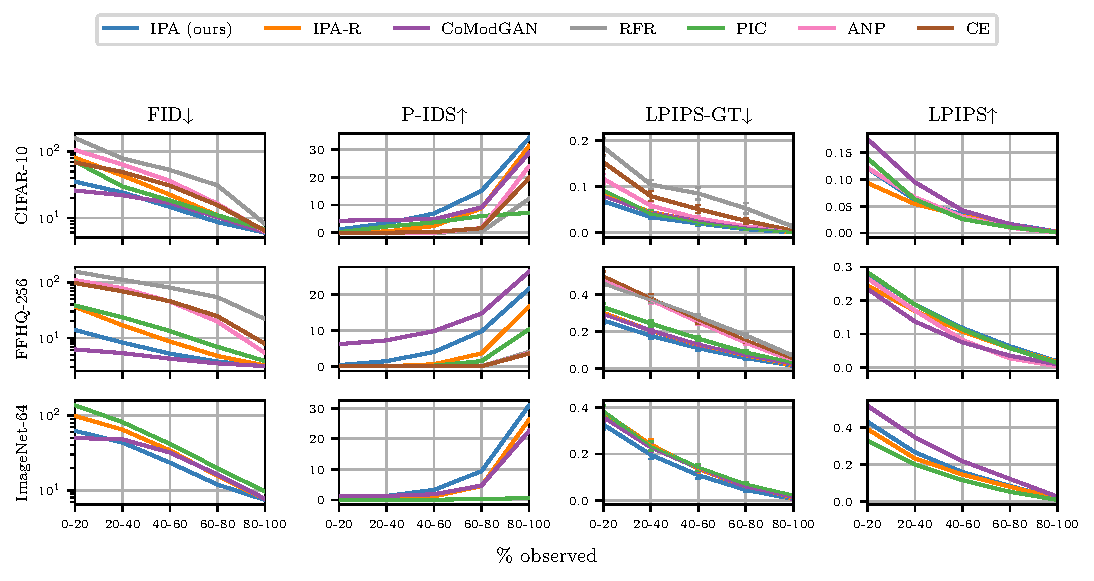
\includegraphics[width=\textwidth]{figs/cigcvae/extra-metrics}
  \caption{Expanded \cref{fig:cigcvae-metrics} including results on ImageNet-64 and the
    LPIPS diversity score.}
  \label{fig:cigcvae-extra-metrics}
\end{figure}

\begin{figure}
  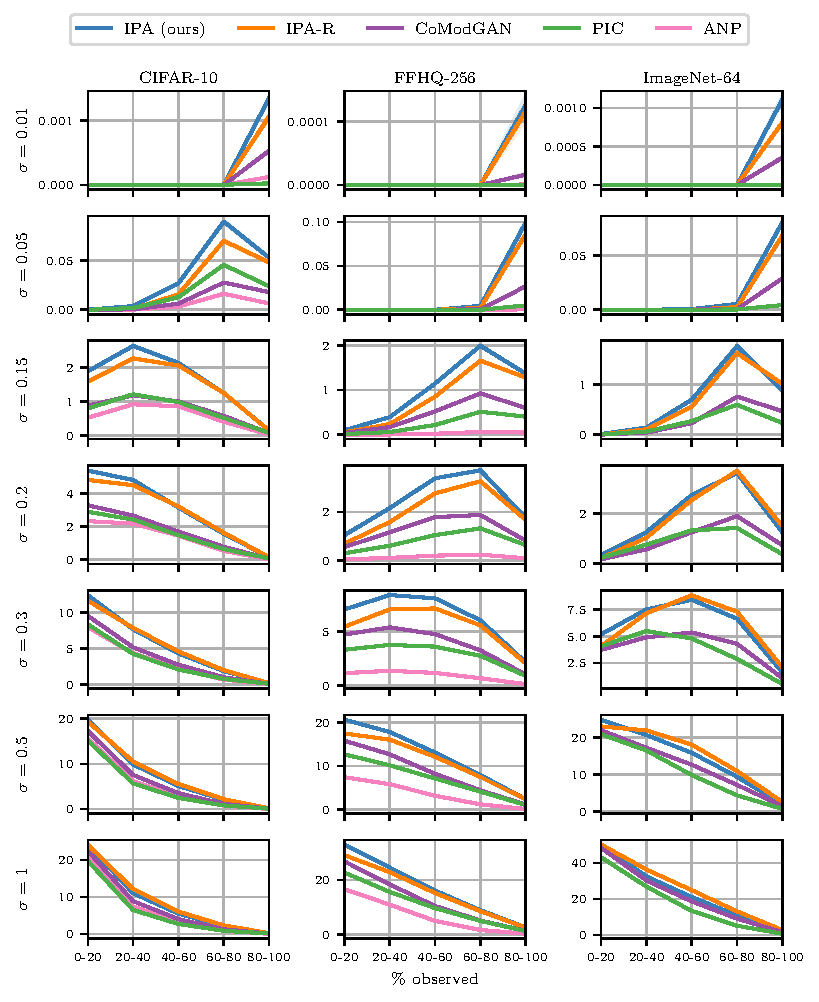
\includegraphics[scale=1]{figs/cigcvae/fwv_sigma}
  \caption{The faithfulness weighted variance for inpainting on CIFAR-10,
    FFHQ-256, and ImageNet-64, for various values of $\sigma$. IPA obtains the
    best performance on almost all datasets and values of $\sigma$, only being
    outperformed by IPA-R on CIFAR-10 with high values of $\sigma$. This
    indicates that IPA both assigns high probability density to the ground truth
    (and so performs well for small $\sigma$) and generates diverse samples (and
    so performs well for larger $\sigma$).}
  \label{fig:cigcvae-fwv}
\end{figure}



\section{Bayesian optimal experimental design} \label{sec:cigcvae-supp-boed}

\subsection{EIG estimators}  \label{sec:cigcvae-eig-estimator}

In this section, we expand on how our estimator for the expected information
gain differs from prior work~\citep{harvey2019near}. Repeating some relevant
definitions from the main text, $f_{\coord{}_1,\ldots,\coord{}_t}$ is a function which maps
from a full image to a sequence of observations of the image at locations
$\coord{}_1,\ldots,\coord{}_t$. When estimating the EIG at time step $t$, we will have already
observed a sequence of observations denoted $\partI{}_{\coord{}_1,\ldots,\coord{}_{t-1}}$,
extracted from some latent image $\I{}$ as $f_{\coord{}_1,\ldots,\coord{}_{t-1}}(\I{})$. We
use a CNN which outputs $g(v|f_{\coord{}_1,\ldots,\coord{}_t}(\I{}))$, an approximation of the
posterior over the latent variable of interest given a sequence of observations.
Following \citet{harvey2019near}, we will from now on refer to this as the
AVP-CNN (attentional variational posterior CNN).
%
Both our method and that of \citet{harvey2019near} sample image completions,
which we denote $\I{}^{(1)},\ldots,\I{}^{(N)}$, conditioned on
$\partI{}_{\coord{}_1,\ldots,\coord{}_{t-1}}$. \citet{harvey2019near} do so by retrieving
images which roughly match the observed pixel values from a database. Although
completions from this are diverse, they can match the observed values poorly. We
therefore replace this stage with an image completion network trained using
IPA.

Given these components, \citet{harvey2019near} approximate the expected
information gain with
\begin{align}
  \label{eq:old-eig}
  \text{EIG}(\coord{}_t; \partI{}_{\coord{}_1,\ldots,\coord{}_{t-1}}) &\approx \overbrace{\mathcal{H} \left[ g(\cdot|\partI{}_{\coord{}_{1},\ldots,\coord{}_{t-1}}) \right]}^{\text{entropy after $t-1$ scans}} - \overbrace{\frac{1}{N} \sum_{n=1}^N  \mathcal{H} \left[ g(\cdot|f_{\coord{}_1,\ldots,\coord{}_t}(\I{}^{(n)})) \right]}^{\text{expected entropy after $t$ scans}}.
\end{align}
Since the prior entropy term of \cref{eq:old-eig} does not depend on $\coord{}_t$, it
can be neglected when choosing $\coord{}_t$ with BOED. As only the expected posterior
entropy then needs to be estimated and compared for various $\coord{}_t$, we will from
now on refer to this estimator with the acronym EPE (for `expected posterior
entropy').

We use a different estimator for the prior entropy. It becomes equivalent as $N
\rightarrow \infty$ if $g$ and the image completion method are perfect but, when
this is not the case, produces an estimate of the prior entropy with a
dependence on $\coord{}_t$. To repeat \cref{eq:new-eig}, this results in the following
estimator for the EIG:
\begin{align}
  \label{eq:new-eig-supp}
  \text{EIG}(\coord{}_t;& \partI{}_{\coord{}_1,\ldots,\coord{}_{t-1}}) \approx \overbrace{\mathcal{H} \left[ \frac{1}{N} \sum_{n=1}^N g(\cdot|f_{\coord{}_1,\ldots,\coord{}_t}(\I{}^{(n)})) \right]}^{\text{entropy after $t-1$ scans}} - \overbrace{\frac{1}{N} \sum_{n=1}^N  \mathcal{H} \left[ g(\cdot|f_{\coord{}_1,\ldots,\coord{}_t}(\I{}^{(n)})) \right]}^{\text{expected entropy after $t$ scans}}.
\end{align}
While it is not immediately clear that this estimator is better than that in
\cref{eq:old-eig}, one useful property is that, like the true expected
information gain, it is guaranteed to be non-negative. This can be seen as
follows. First, note that the prior entropy term is the entropy of an
expectation (over $n \sim \text{Uniform}(1, N)$), and the expected posterior
entropy term swaps the order of the entropy and expectation. Since the mapping
from a distribution $g(\cdot)$ to its entropy $\mathcal{H}[g(\cdot)]$ is
strictly concave, Jensen's inequality is applicable. Invoking Jensen's
inequality shows that the prior entropy term must be greater than or equal to
the expected posterior entropy, and so the estimate of the EIG will be
non-negative. In \cref{fig:cigcvae-boed-auroc-supp}, we compare the performance of this
estimator (denoted EIG) and that in \cref{eq:old-eig} (EPE). We find that the
estimator denoted EIG leads to significantly better classification performance.

Another view of our EIG estimator is as a variant of the inception
score~\citep{salimans2016improved} for the sampled images
$\I{}^{(1)},\ldots,\I{}^{(N)}$. The standard inception score is computed using
an image classifier trained on ImageNet~\citep{salimans2016improved}.
\Cref{eq:new-eig} is the inception score if this classifier is replaced with the
AVP-CNN acting on observations of each image at locations $\coord{}_1,\ldots,\coord{}_t$.

\begin{figure*}[t]
  \centering
  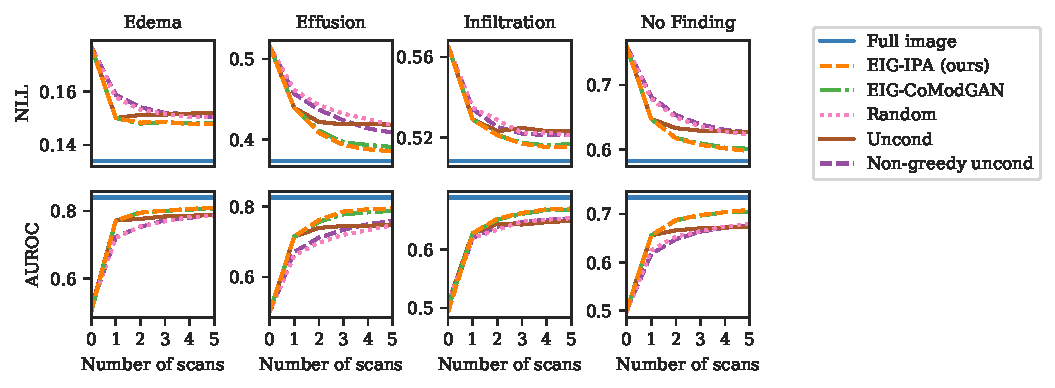
\includegraphics[width=\textwidth]{figs/cigcvae/boed-auroc-curve-supp}
  \caption{We extend on \cref{fig:cigcvae-boed} by additionally reporting negative
    log-likelihoods (top row) for the classification tasks. We also include
    results from the `EPE' estimator used by \citet{harvey2019near}. We see that
    our BOED estimator provides significant improvements; resulting performance
    is always superior to the other baselines. This is only sometimes the case
    for the `EPE' estimator. }
  \label{fig:cigcvae-boed-auroc-supp}
\end{figure*}

\begin{figure}[t]
  \centering
  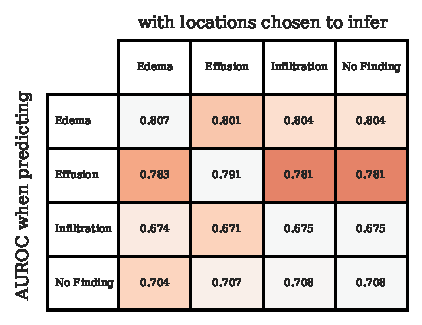
\includegraphics[scale=1]{figs/cigcvae/table-AUROC-boed}
  \caption{AUROC scores when performing one classification task with scan
    locations chosen for a different classification task. The intensity of the
    colour of each cell is proportional to the difference between its value and
    the greatest value in its row.}
  \label{fig:cigcvae-boed-correlations}
\end{figure}

\subsection{BOED baselines}
\paragraph{Random}
This baseline simply samples the scan location independently at each time step
from a uniform distribution over all valid locations.

\paragraph{Uncond}
This baseline ablates our estimator for the EIG (\cref{eq:new-eig}) by sampling
images $\I{}^{(1)},\ldots,\I{}^{(N)}$ from the training dataset (without
conditioning on $\partI{}_{\coord{}_1,\ldots,\coord{}_{t-1}}$) instead of from IPA
(conditioned on $\partI{}_{\coord{}_1,\ldots,\coord{}_{t-1}}$). That is, we use:
\begin{align}
  \label{eq:uncond}
  \text{U}^{\text{uncond}}(\coord{}_t; \coord{}_1,&\ldots,\coord{}_{t-1}) = \mathcal{H} \left[ \frac{1}{N} \sum_{n=1}^N g(\cdot|f_{\coord{}_1,\ldots,\coord{}_t}(\I{}^{(n)})) \right] - \frac{1}{N} \sum_{n=1}^N  \mathcal{H} \left[ g(\cdot|f_{\coord{}_1,\ldots,\coord{}_t}(\I{}^{(n)})) \right]
\end{align}
with $\I{}^{(1)},\ldots,\I{}^{(N)} \sim p(\I{})$. The resulting choice of scan
location $\coord{}_t$ at each time step $t$ has no dependence on previous
observations $\partI{}_{\coord{}_1,\ldots,\coord{}_{t-1}}$.

\paragraph{Non-greedy uncond}
When selecting scan locations that optimise the EIG, we select the scan location
at each time step greedily to optimise the EIG from the next scan. To do
otherwise (i.e.~maximise the EIG from multiple next scans) is intractable
because of the dependence of the EIG at each $t$ on previous observations
$\partI{}_{\coord{}_1,\ldots,\coord{}_{t-1}}$. However, since the above `Uncond' baseline
selects each $\coord{}_t$ independently of what is observed at previous scans, we can
remove this greedy property. We do so by selecting all $\coord{}_1,\ldots,\coord{}_T$
simultaneously to maximise
\begin{align}
  \text{U}^{\text{non-greedy}}(\coord{}_1,&\ldots,\coord{}_T) = \mathcal{H} \left[ \frac{1}{N} \sum_{n=1}^N g(\cdot|f_{\emptyset}(\I{}^{(n)})) \right] - \frac{1}{N} \sum_{n=1}^N  \mathcal{H} \left[ g(\cdot|f_{\coord{}_1,\ldots,\coord{}_T}(\I{}^{(n)})) \right]
\end{align}
with $\I{}^{(1)},\ldots,\I{}^{(N)} \sim p(\I{})$. Since the number of possible
values of $\coord{}_1,\ldots,\coord{}_T$ increases exponentially with $T$, it is not feasible
to search over all of them. We therefore optimise this sequence by
randomly sampling a set of such sequences, and choosing the best from this set.


\begin{figure*}[p]
  \centering
  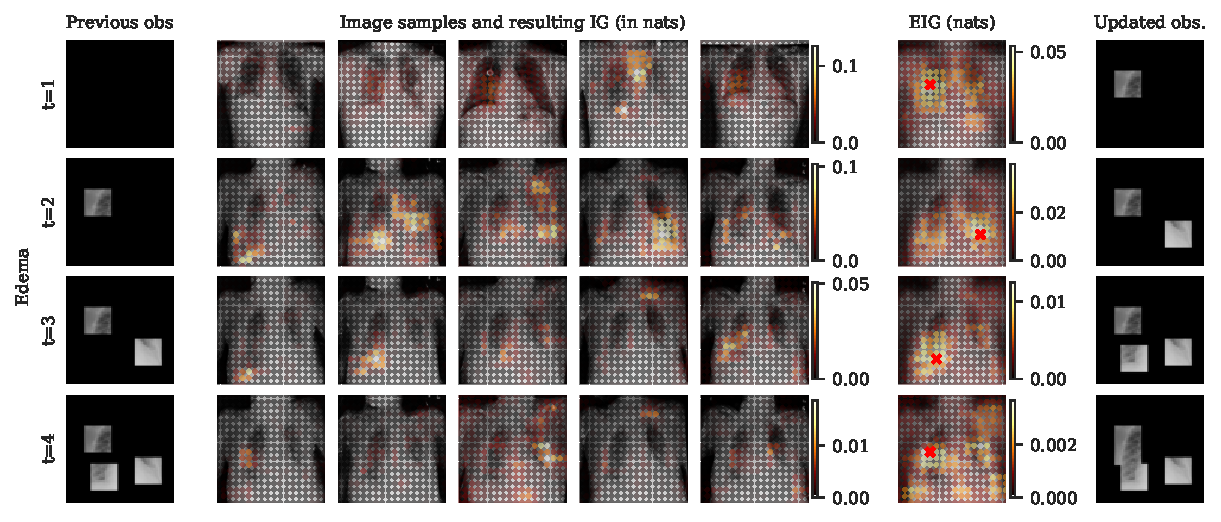
\includegraphics[width=0.98\textwidth]{figs/cigcvae/boed-visualisation-4960-compressed.pdf}
  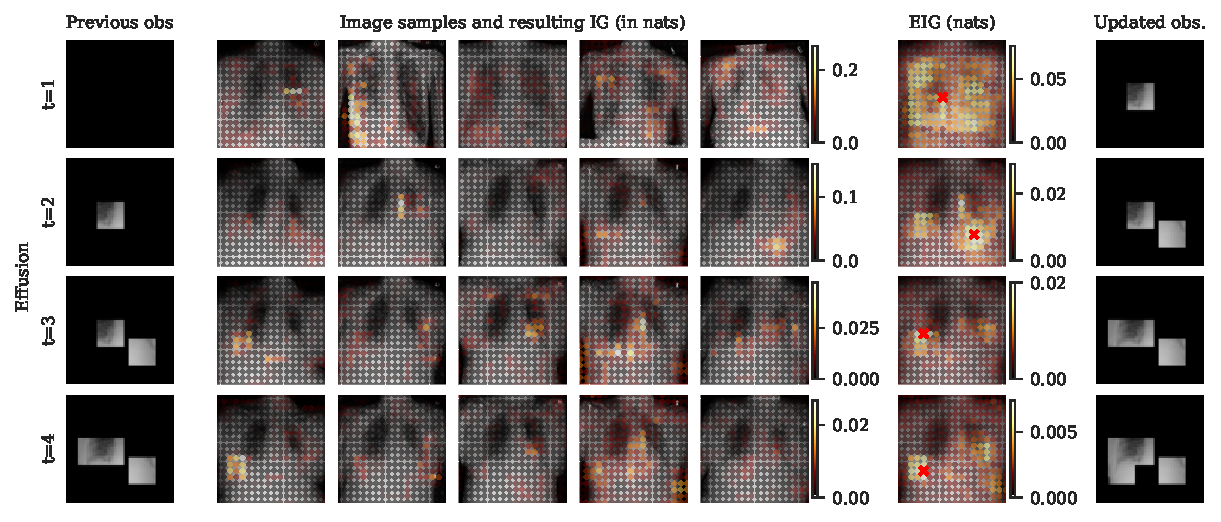
\includegraphics[width=0.98\textwidth]{figs/cigcvae/boed-visualisation-4970-compressed.pdf}
  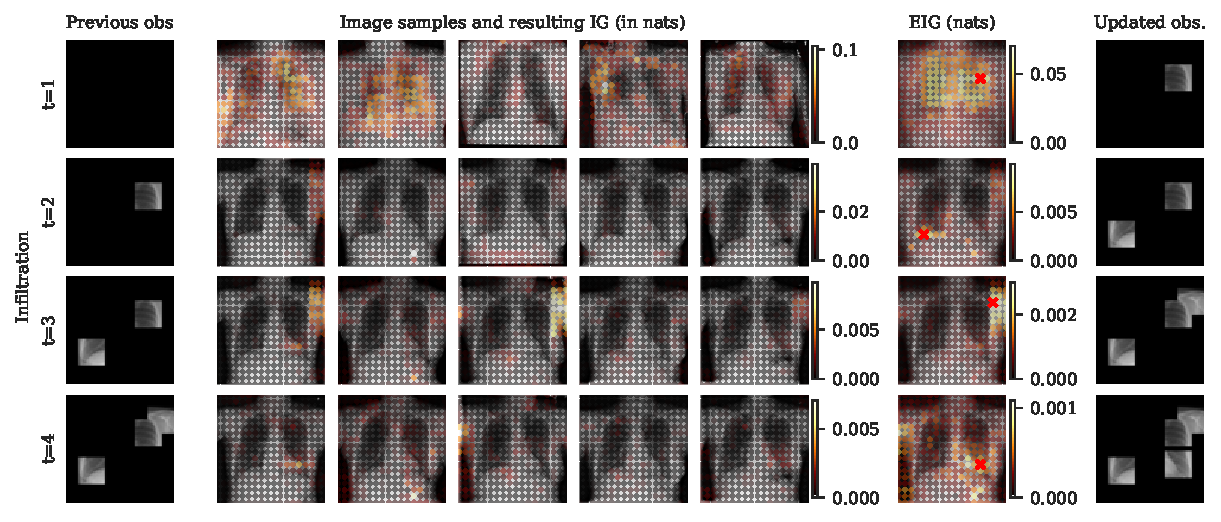
\includegraphics[width=\textwidth]{figs/cigcvae/boed-visualisation-4980-compressed.pdf}
  \caption{Visualisations of BOED processes. On the top, the task is to detect
    `Edema'. In the middle, we aim to detect `Effusion' in a different patient.
    The task at the bottom is to detect `Infiltration'. Four scan locations are
    selected for each. The left column shows the observations made before
    selecting each scan location. The next five columns show five of the $N=10$
    sampled image completions conditioned on these observations. Each is
    overlaid with the information gain predicted after scanning any location.
    The second column from the left shows the expected information gain at each
    location, given by averaging the information gains arising from each sampled
    image completion. A red cross marks the maximum. The final column shows the
    updated observations after scanning the location which maximises the
    expected information gain.}
  \label{fig:cigcvae-extra-xray-boed}
\end{figure*}

\subsection{Additional BOED results} \label{supp:cigcvae-boed-results}
\Cref{fig:cigcvae-boed-auroc-supp} shows additional results from classification with
sequences chosen by BOED and our baselines. In particular, we report negative
log-likelihoods for the class labels as well as the AUROC scores. We see that
the negative log-likelihood sometimes increases as more scans are taken,
indicating that the classifier used is not perfectly trained. Interestingly,
this only happens when glimpses are chosen with the EPE estimator of
\citet{harvey2019near}. This may be because the EPE estimator has a tendency to
select locations which cause the classifier to be overconfident (and thus
produce artificially low posterior entropies). With the EIG estimator, and the
baselines, this issue is not observed.

To illustrate that the scan locations chosen by BOED are task-dependent,
\cref{fig:cigcvae-boed-correlations} shows the results from using scan locations chosen
for one classification task (i.e.~diagnosing a particular disease) to perform a
different classification task. Each row shows the results for a particular task,
with each column showing results when scan locations are chosen based on a
particular task. As expected, the highest (or at least joint-highest) AUROC
score in each row occurs on the diagonal, when the classification task and
choice of scan locations are aligned. Away from the diagonal, the scores are
only slightly lower, perhaps reflecting that there is a large overlap between
the relevant areas for these tasks.

\Cref{fig:cigcvae-extra-xray-boed} shows additional visualisations of the Bayesian
experimental design process for different test images, adding to the one shown
in the main paper. The `information gains' shown for a particular $\I{}^*$
(sampled conditioned on observations $\partI{}_{\coord{}_1,\ldots,\coord{}_{t-1}}$) are
computed as the following KL divergence:
% EIG but the `expected
% entropy after $t$ scans' term is replaced by the entropy given a particular
% sampled $\I{}^*$. That is,
\begin{align}
  \label{eq:ig}
                                                   \text{IG}(\I{}^*, \coord{}_t; \partI{}_{\coord{}_1,\ldots,\coord{}_{t-1}}) \approx \kl[\Bigg]{g(\cdot|f_{\coord{}_1,\ldots,\coord{}_t}(\I{}^*))}{\frac{1}{N} \sum_{n=1}^N g(\cdot|f_{\coord{}_1,\ldots,\coord{}_t}(\I{}^{(n)}))}.
\end{align}
Crucially, averaging information gains computed with $\I{}^*=\I{}^{(1)}$ to
$\I{}^{(N)}$ gives the estimate of the EIG presented in \cref{eq:new-eig}.

\subsection{BOED experimental details}
The AVP-CNN, $g$, is trained to map from masked images, $\partI{}$, to
distributions over the class labels. Each image in the Chest X-ray 14 dataset
has labels indicating the presence or absence of each of 14 pathologies. We
train $g$ to produce 15 outputs: an estimated probability of the presence or
absence of each of the 14 conditions individually; and an additional estimate of
the probability that any (one or more) of these conditions is present. We train
$g$ to estimate these using a cross-entropy loss. Masked images are sampled
using almost the same mask distribution as for training the image completion
networks (described in \cref{sec:cigcvae-experiments}); the only difference is that
patches now have 25\% rather than 35\% of the image width, to match the
observations we use in the experiments with BOED. We use an AVP-CNN pretrained
on ImageNet and then trained on Chest X-ray 14 for 32\,000 iterations with a
batch size of 32 and learning rate $1\times10^{-5}$. We train IPA as described
in \cref{supp:cigcvae-exp-details}.

We select each scan location by evaluating \cref{eq:new-eig} at every point in
an evenly-spaced $17\times17$ grid over the image, and choosing the maximum. We
evaluate the EIG with $N=10$ sampled image completions. This is repeated to
select the scan location for each $t=1,\ldots,5$ (with the sampled images
conditioned on observations up to $t-1$ at each stage). Where applicable, we use
the same trained networks and hyperparameters for the baselines. For the
`non-greedy uncond' baseline, we select a scan location sequence by choosing the
best of 289 sampled sequences. This number was chosen to match the number of
locations in the $17\times17$ grid that the other methods search over at each
time step. The results reported in \cref{fig:cigcvae-boed,fig:cigcvae-boed-auroc-supp} were
computed on a randomly-sampled 5000 image subset of the Chest X-ray 14 test set.


\section{Out-of-distribution detection} \label{supp:cigcvae-ood} A major advantage of
likelihood-based models is the possibility to use them to detect when an input
is dissimilar to the training data (out-of-distribution, or OOD). Since a
learned model is likely to perform poorly on such inputs, it is important for
deployed systems to be able to recognise them and this has been the focus of a
substantial body of
work~\citep{ren2019likelihood,hendrycks2016baseline,xiao2020likelihood,havtorn2021hierarchical}.
The task we consider is detecting whether a partially observed image (e.g.~the
input to an image completion system) is OOD.


\begin{figure}[t]
    \footnotesize
  \centering
  \begin{minipage}{0.41\textwidth}

    \centering
    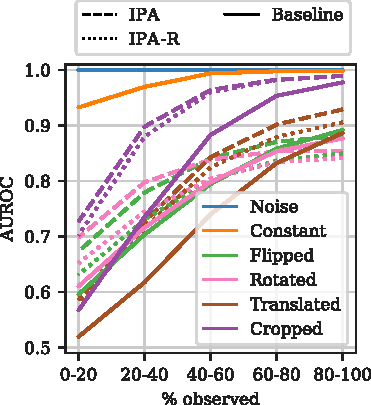
\includegraphics[scale=.8]{figs/cigcvae/ood-ffhq}

  \end{minipage}
  \begin{minipage}{.58\textwidth}

%  \caption{AUROC scores for OOD detection. Higher is better.}
  \begin{tabular}{lccccc}
    \toprule
    ID & \multicolumn{5}{c}{CIFAR-10}  \\
    \cmidrule(r){2-6}
    OOD & Noise & Const. & Flip & Rotate & SVHN \\
    \midrule
    IPA      & \textbf{.995} & \textbf{.949} & \underline{.552} & \underline{.594} & \textbf{.753}    \\
    IPA-R    & .987         & \underline{.921}                  & \textbf{.635}    & \textbf{.619}    & \underline{.686} \\
    Baseline  & \underline{.993} & .909 & .543             & .536             & .556             \\
    \bottomrule
  \end{tabular}
  \newline
  \vspace*{.1cm}
  \newline
  \begin{tabular}{lcccccc}
    \toprule
    ID & \multicolumn{5}{c}{FFHQ-256}  \\
    \cmidrule(r){2-6}
    OOD         & Noise & Const. & Flip & Rotate & ~Crop~ \\
    \midrule
    IPA         & \textbf{1.00} & \textbf{1.00} & \textbf{.809}    & \textbf{.808}    & \textbf{.912}    \\
    IPA-R       & \textbf{1.00} & \textbf{1.00} & \underline{.770} & \underline{.775} & \underline{.902} \\
    Baseline     & \textbf{1.00} & 0.98  & .769 & .771             & .823             \\
    \bottomrule
  \end{tabular}

\end{minipage}%
\caption{OOD-detection on incomplete images. On the left, we show AUROC scores
  on FFHQ-256 computed separately for masks from varying distributions. On the
  right we report, for both CIFAR-10 and FFHQ-256, the average of these scores
  over all mask distributions.}
\label{fig:cigcvae-ood-results}
% \vspace{-.5cm}
\end{figure}

OOD-detection using probabilistic models is theoretically appealing and robust,
since no assumptions need to be made about the OOD
data~\citep{xiao2020likelihood,havtorn2021hierarchical}. Such OOD-detection
metrics commonly have the following interface: they take as input a
probabilistic model (e.g.~a VAE) and a data point, and output a scalar value.
The greater the value of this scalar, the more likely it is that the data point
is within the distribution of the generative model. One intuitive metric is
simply the log-likelihood of the data point under the model. This can work
poorly in practice, however, and it has been found that learned models sometimes
assign higher likelihood to out-of-distribution data than to in-distribution
data~\citep{nalisnick2018deep}. Several alternative OOD-detection metrics have
been proposed specifically for
VAEs~\citep{xiao2020likelihood,havtorn2021hierarchical}. To use them, we note
that we can use networks trained with either IPA or IPA-R to lower-bound the
likelihood of a partially-observed image. Specifically, this lower-bound is the
reverse KL objective in \cref{eq:reverse-obj}. After conducting preliminary
experiments using the VD-VAE with several OOD-detection
metrics~\citep{xiao2020likelihood,havtorn2021hierarchical}, we found that
\begin{wrapfigure}[18]{R}{.4\textwidth}
  \vspace{-.4cm}
  \centering
  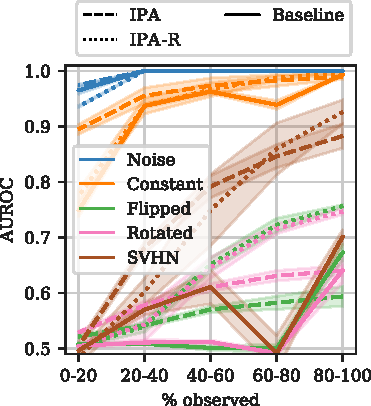
\includegraphics[scale=.8]{figs/cigcvae/ood-supplementary}
  \caption{Breakdown of AUROC for each mask distribution on CIFAR-10. }
  \label{fig:cigcvae-ood-supplementary}
\end{wrapfigure}
improved performance could be obtained (for OOD-detection of both partially- and
fully-observed images) using the ``temperature gradient'' metric described
further in \cref{supp:cigcvae-temp-grad} below.
%
It is efficient to compute, requiring the VAE to be run just once and gradients
computed.

As a baseline, we complete the partially observed image with our best performing
baseline image completion method, CoModGAN, and perform OOD-detection on the
result (using the ``temperature gradient'' metric on an unconditional VD-VAE).
\Cref{fig:cigcvae-ood-results} shows our results on CIFAR-10 and FFHQ-256. We test
various types of OOD data: \textbf{Noise} samples each pixel value independently
from a uniform distribution; \textbf{Constant} uniformly samples a single colour
for the entire image; \textbf{Flip} vertically flips an in-distribution (ID)
image; \textbf{Rotate} rotates an ID image by 90$^{\circ}$; \textbf{Crop}
upsamples an ID image by a factor of 1.5 and then crops to the original size.
\textbf{SVHN} is the Street View House Number dataset~\citep{netzer2011reading}.
With 80-100\% of the image observed, we obtain better AUROCs than similar
methods applied to the full image. In particular, on CIFAR-10 vs SVHN, we
outperform both \citet{xiao2020likelihood} and \citet{havtorn2021hierarchical},
albeit with a larger VAE architecture. Using IPA for OOD-detection results in
performance that degrades gracefully as less of the image is observed. There are
therefore particularly large benefits over the baseline when only 0-20\% or
20-40\% of the image is observed.

\Cref{fig:cigcvae-ood-supplementary} shows a breakdown of the AUROC scores for each mask
distribution on CIFAR-10, similar to that shown for FFHQ-256 in
\cref{fig:cigcvae-ood-results}. Error bars are standard deviations computed with 3 runs,
with the unconditional VD-VAE and IPA/IPA-R retrained each time.



\subsection{Out-of-distribution detection with temperature gradients} \label{supp:cigcvae-temp-grad}


We conducted preliminary experiments with several techniques for OOD-detection
with VAEs, applying each to the VD-VAE architecture. Using the likelihood-regret
technique~\citep{xiao2020likelihood} with the VD-VAE is computationally costly
(as it involves optimising neural network parameters), and we obtained results
on CIFAR-10 considerably worse than those produced by the smaller VAE
architecture with which it was introduced. We also implemented the
log-likelihood ratio metric \citep{havtorn2021hierarchical} for the VD-VAE, but
did not find any hyperparameter configurations with which it was consistently
better than random guessing across different tasks.

We therefore introduce a metric which we found to work well with the VD-VAE. It
is based on a common heuristic to make a VAE produce more regular samples:
reducing the variance of the prior over its latent
variables~\citep{vahdat2020nvae}. If $\mathbf{t}$ is a vector containing the
temperature $\mathbf{t}_l$ for each layer $l$, then doing so corresponds to
modifying the prior $\pmodel{}(\z{})$ so that the Gaussian distribution over each
group of latent variables is scaled by the corresponding temperature:
\begin{equation}
  \pmodel{}(\z{}; \mathbf{t}) = \prod_{l=1}^L  \frac{1}{C(\mathbf{t}_l, \z{}_{<l})} \pmodel{}(\z{}_l|\z{}_{<l})^{\frac{1}{\mathbf{t}^2_l}}
\end{equation}
where $C(\mathbf{t}_l, \z{}_{<l})$ is a normalisation constant. In practice, since
$\pmodel{}(\z{}_l|\z{}_{<l})$ is a Gaussian distribution, this scaling corresponds to
simply multiplying the standard deviation by $\mathbf{t}_l$.

We can lower-bound the corresponding marginal likelihood $\pmodel{}(\partI{};
\mathbf{t})$ using the partial encoder similarly to the training objective in
\cref{eq:reverse-obj}:
\begin{align}
  \EX_{\pdata{}(\partI{})} \left[ \log \pmodel(\partI{}; \mathbf{t}) \right] \geq \EX_{\pdata{}(\partI{})}\EX_{\partq{}(\z{}|\partI{})} \left[ \log\frac{\pmodel{}(\z{}; \mathbf{t})\pmodel{}(\partI{}|\z{})}{\partq{}(\z{}|\partI{})} \right] .
\end{align}
We hypothesise that OOD examples will usually either be excessively regular, and
therefore have a higher marginal likelihood for $t<1$, or excessively irregular,
and therefore have a higher likelihood for $t>1$. In-distribution (ID) examples,
on the other hand, should have the highest marginal likelihood for $t\approx 1$.
A useful feature to distinguish between ID and OOD examples is therefore likely
to be the gradient $\frac{\partial}{\partial\mathbf{t}}p(\partI{};
\mathbf{t})\lvert_{\mathbf{t}=\mathbf{1}}$, which we can approximate with the
gradient w.r.t. $\mathbf{t}$ of the lower-bound above. We fit a multivariate
Gaussian to 5000 samples of
$\frac{\partial}{\partial\mathbf{t}}p(\partI{}^{(i)};
\mathbf{t})\lvert_{\mathbf{t}=\mathbf{1}}$ with $\partI{}^{(i)}$ sampled from
the training data with the training mask distribution. To obtain a score for how
in-distribution a new example $\partI{}$ is, we compute the probability density
of $\frac{\partial}{\partial\mathbf{t}}p(\partI{};
\mathbf{t})\lvert_{\mathbf{t}=\mathbf{1}}$ under this multivariate Gaussian. The
greater this score, the more likely it is that an example is in-distribution. We
call this the ``temperature-gradient'' metric.

\subsection{OOD detection details} We compute the AUROC scores presented in
\cref{fig:cigcvae-ood-results} using the 5000 image test set for CIFAR-10 and its
OOD-transformations; a 5000 images subset of the SVHN test set; and the 7000
image test set for FFHQ-256. We use 5000 samples of $32\times32$ `Noise' and
`Constant' images when comparing against CIFAR-10, and 200 samples at
$256\times256$ resolution when comparing against FFHQ-256.

We also present results for the `Translated' transformation in
\cref{fig:cigcvae-ood-results} for FFHQ-256. This transformation takes a crop with 90\%
of the image size from one of the four corners and then rescales it to the
original size. The result is thus slightly translated so that e.g.~the eyes of
an FFHQ image are no longer aligned. It is not shown in our results table due to
space constraints.


\section{Lack of semantic diversity in CoModGAN} \label{supp:cigcvae-comodgan-failure}
In this section we demonstrate the some failure cases of CoModGAN in which it
fails to produce semantically diverse images. We suspect that this behaviour of
CoModGAN contributes to its poor performance on the LPIPS-GT metric.
\Cref{fig:cigcvae-comodgan-failure} shows a few examples of partial images for which
CoModGAN struggles to generate semantically diverse images. Compare these
results with IPA's results reported in \cref{fig:cigcvae-comodgan-failure-aipo},
showing a wide range of completions for all the partial images.

\newcommand{\cmgfailureimgheight}{0.8cm}

\begin{figure*}[t]
  \centering
  \begin{subfigure}[t]{0.14\textwidth}
    \centering
    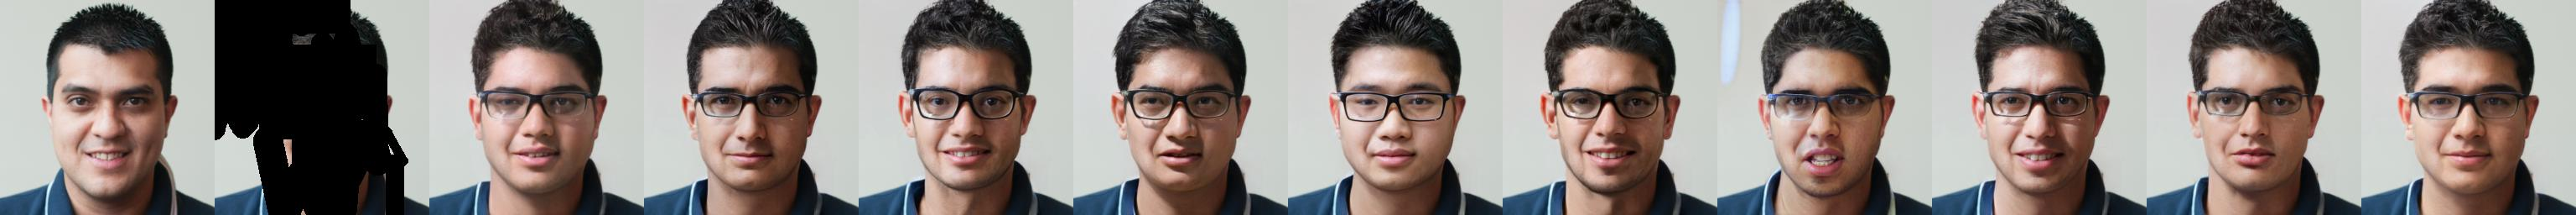
\includegraphics[trim=0px 0px 2560px 0px, clip, height=\cmgfailureimgheight]{figs/cigcvae/co_mod_gan_failure/co_mod_gan_0_3_2.jpg}
    %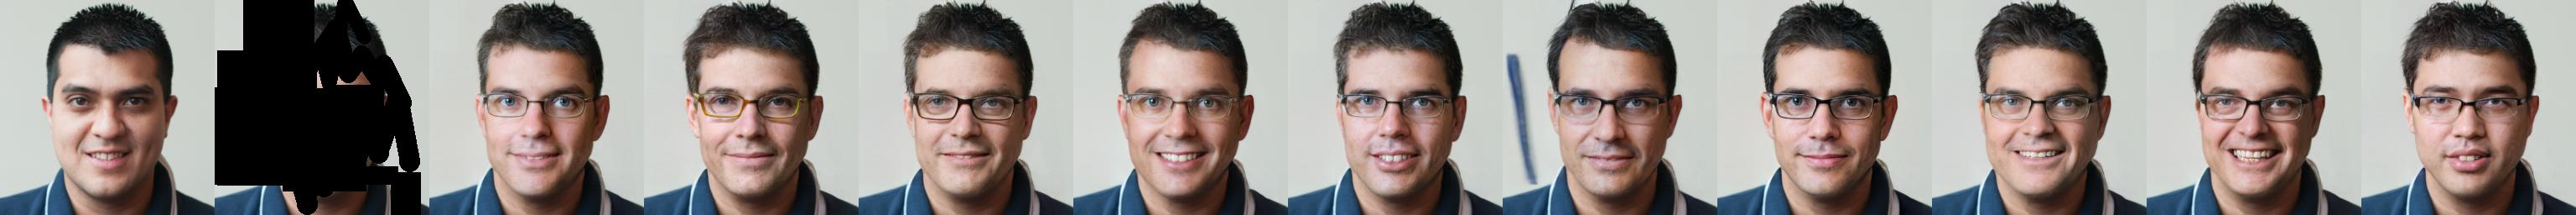
\includegraphics[trim=0px 0px 2560px 0px, clip, height=\cmgfailureimgheight]{figs/cigcvae/co_mod_gan_failure/co_mod_gan_0_3_6.jpg}
    %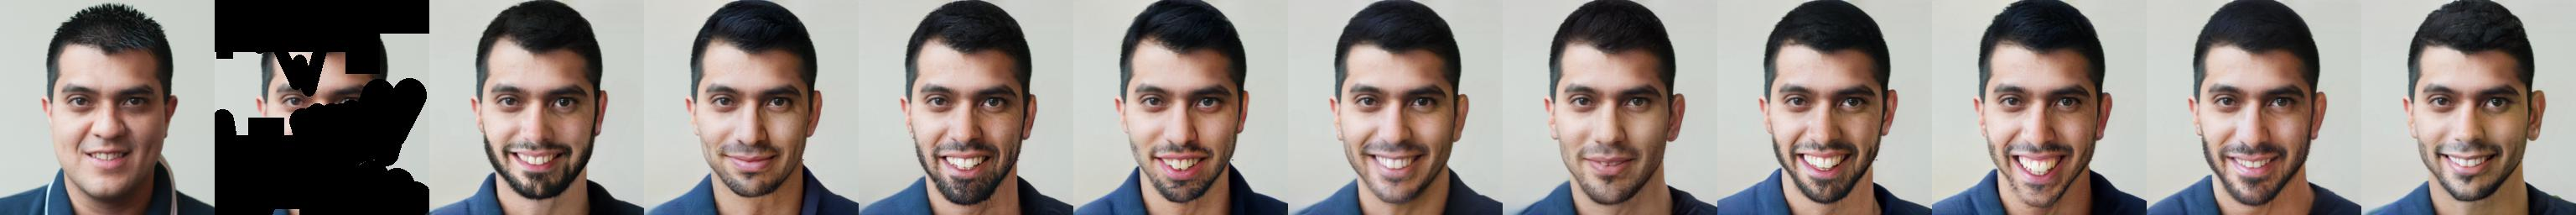
\includegraphics[trim=0px 0px 2560px 0px, clip, height=\cmgfailureimgheight]{figs/cigcvae/co_mod_gan_failure/co_mod_gan_0_3_7.jpg}
    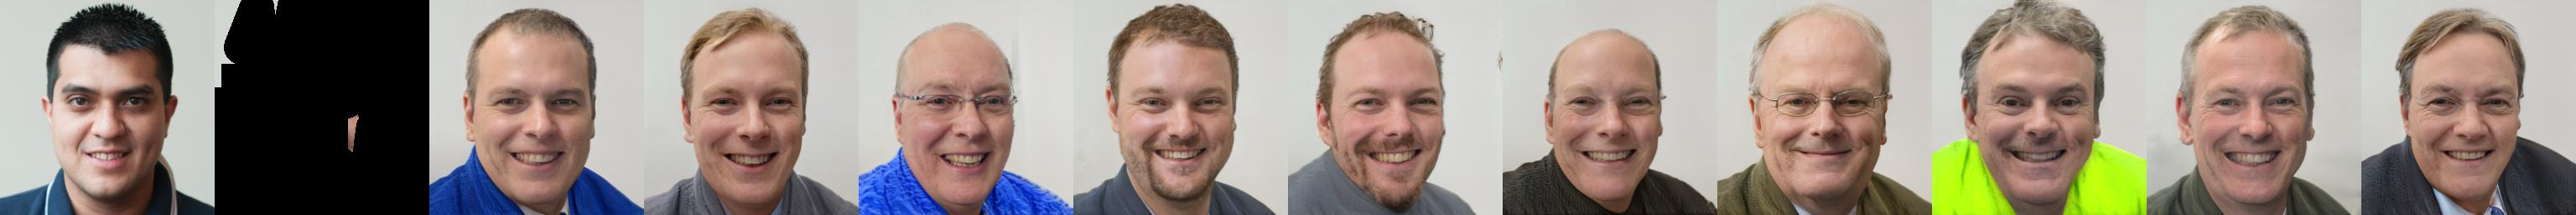
\includegraphics[trim=0px 0px 2560px 0px, clip, height=\cmgfailureimgheight]{figs/cigcvae/co_mod_gan_failure/co_mod_gan_0_4_2.jpg}
    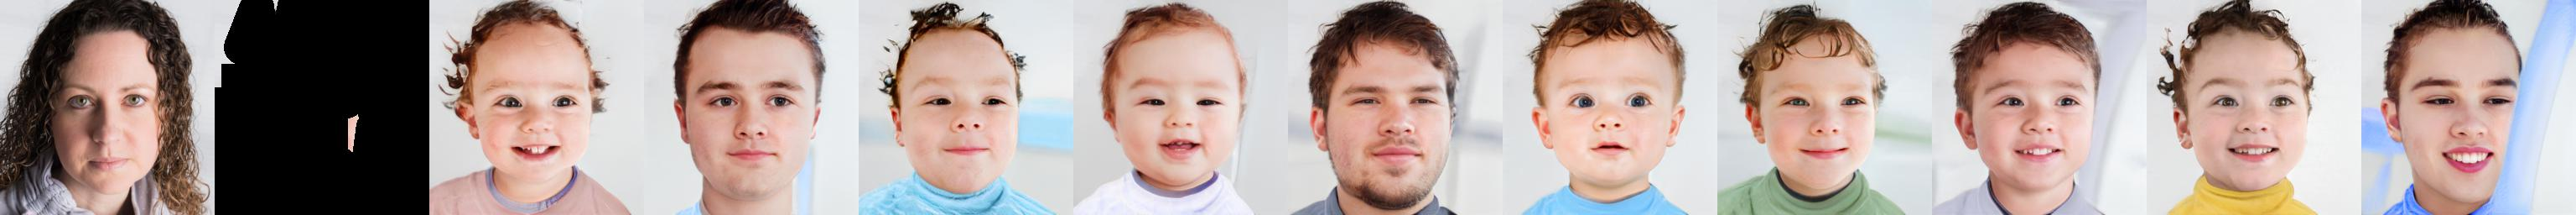
\includegraphics[trim=0px 0px 2560px 0px, clip, height=\cmgfailureimgheight]{figs/cigcvae/co_mod_gan_failure/co_mod_gan_1_4_2.jpg}
    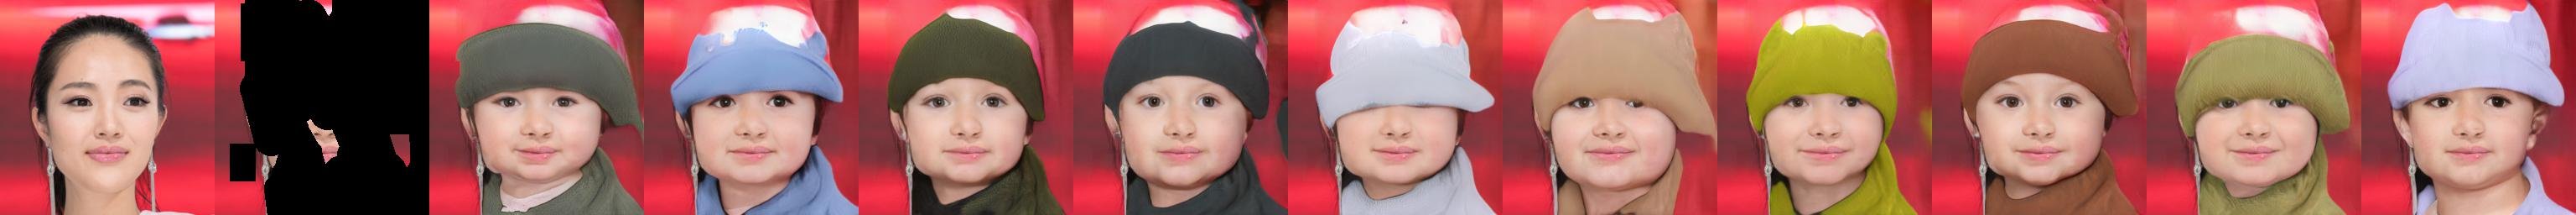
\includegraphics[trim=0px 0px 2560px 0px, clip, height=\cmgfailureimgheight]{figs/cigcvae/co_mod_gan_failure/co_mod_gan_56_4_12.jpg}
    %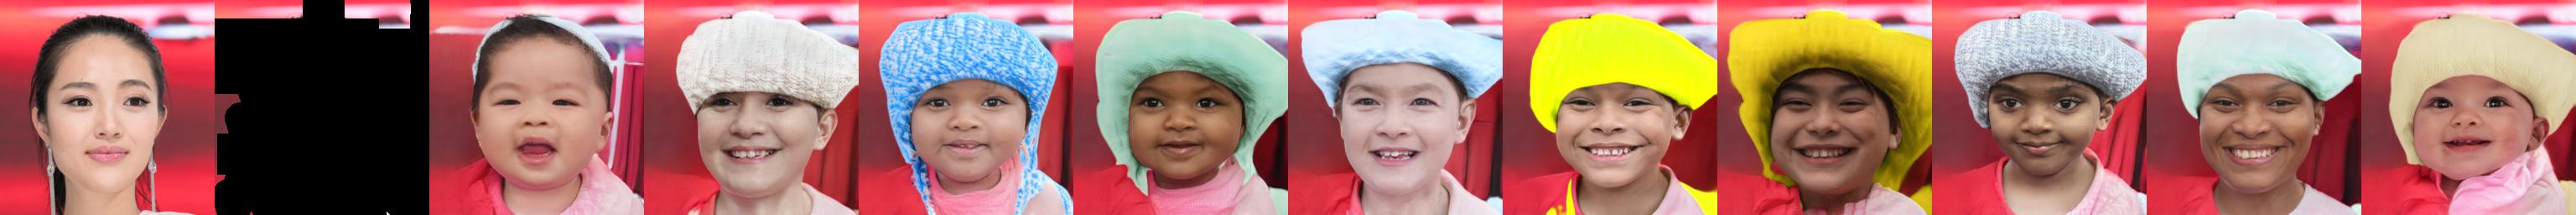
\includegraphics[trim=0px 0px 2560px 0px, clip, height=\cmgfailureimgheight]{figs/cigcvae/co_mod_gan_failure/co_mod_gan_56_4_16.jpg}
    \caption{$\I, \partI$}
  \end{subfigure}
  \begin{subfigure}[t]{0.73\textwidth}
    \centering
    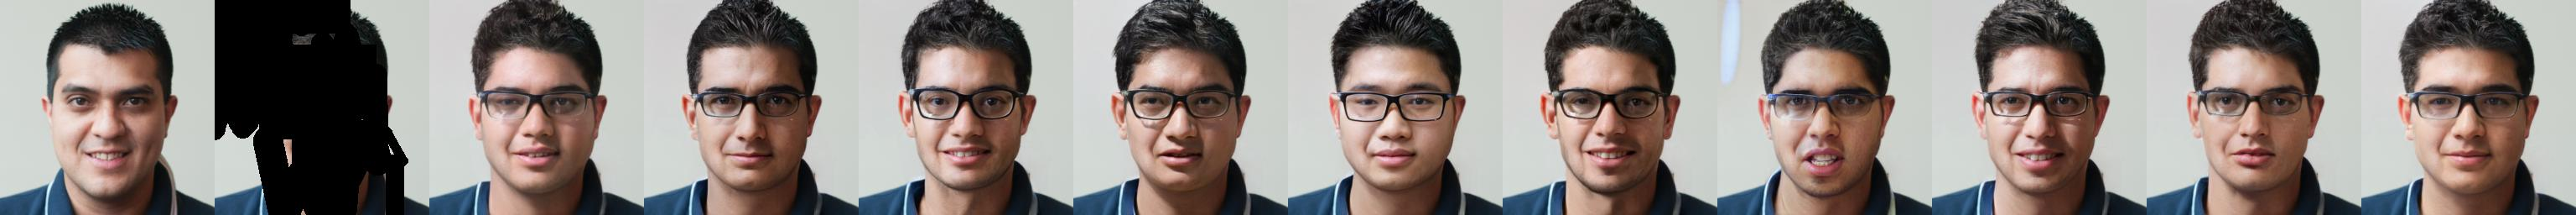
\includegraphics[trim=512px 0px 0px 0px, clip, height=\cmgfailureimgheight]{figs/cigcvae/co_mod_gan_failure/co_mod_gan_0_3_2.jpg}
    %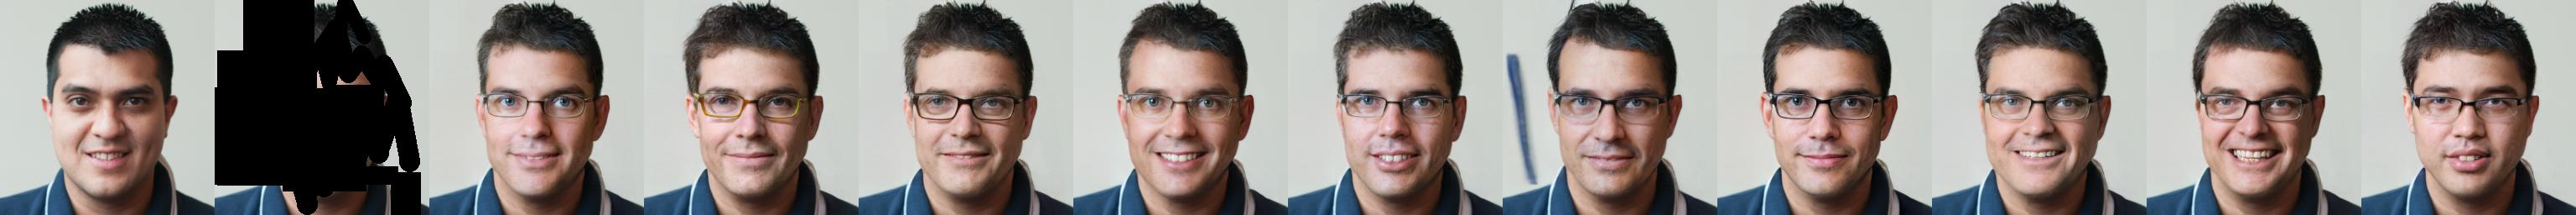
\includegraphics[trim=512px 0px 0px 0px, clip, height=\cmgfailureimgheight]{figs/cigcvae/co_mod_gan_failure/co_mod_gan_0_3_6.jpg}
    %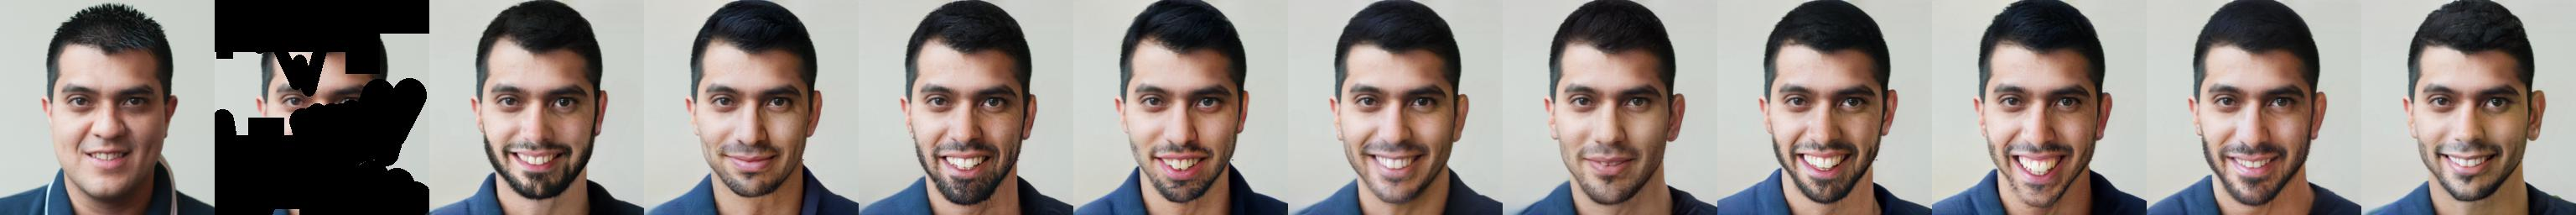
\includegraphics[trim=512px 0px 0px 0px, clip, height=\cmgfailureimgheight]{figs/cigcvae/co_mod_gan_failure/co_mod_gan_0_3_7.jpg}
    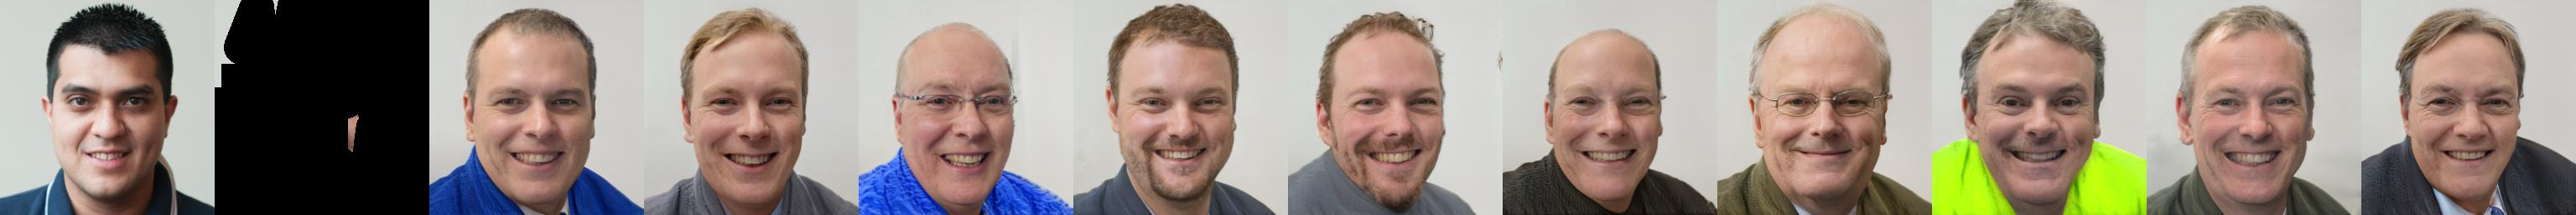
\includegraphics[trim=512px 0px 0px 0px, clip, height=\cmgfailureimgheight]{figs/cigcvae/co_mod_gan_failure/co_mod_gan_0_4_2.jpg}
    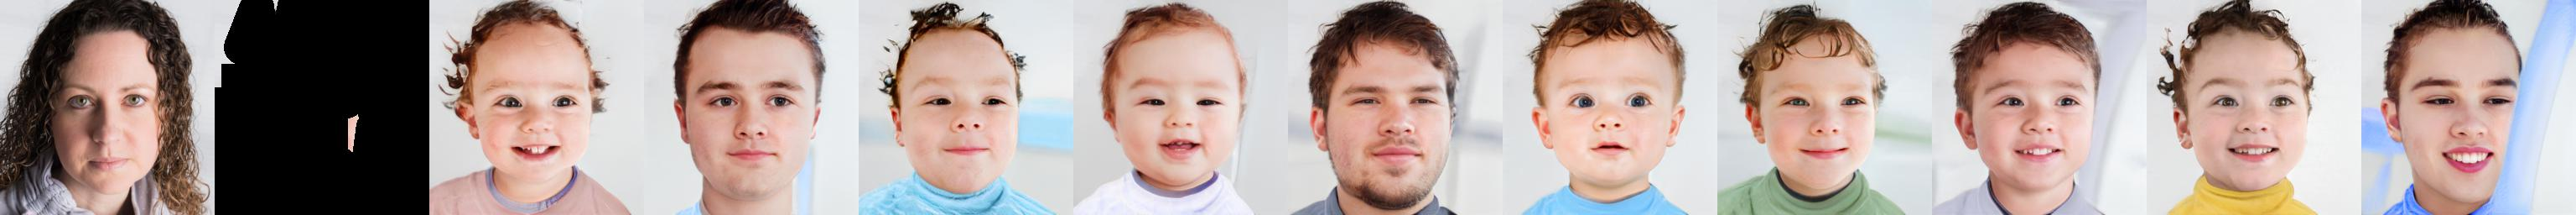
\includegraphics[trim=512px 0px 0px 0px, clip, height=\cmgfailureimgheight]{figs/cigcvae/co_mod_gan_failure/co_mod_gan_1_4_2.jpg}
    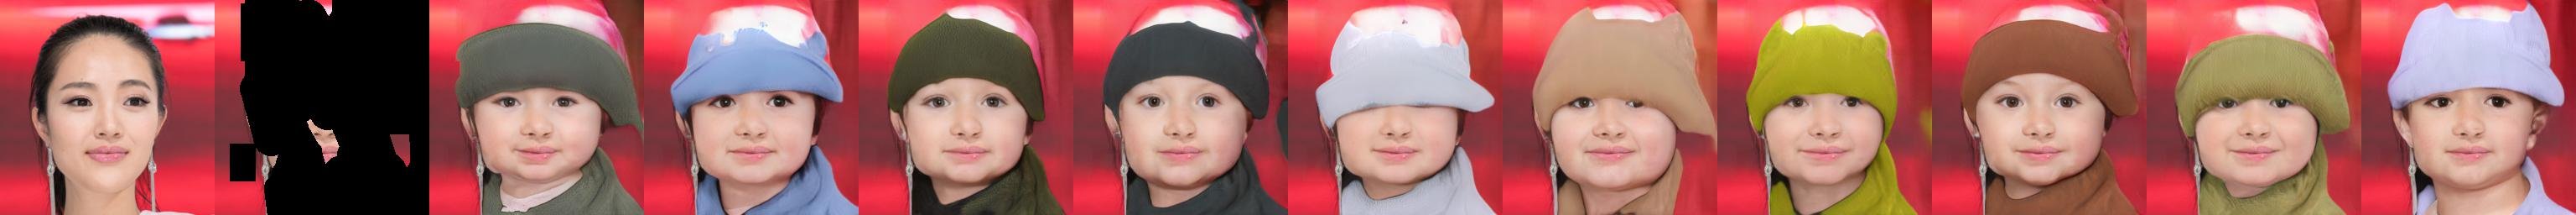
\includegraphics[trim=512px 0px 0px 0px, clip, height=\cmgfailureimgheight]{figs/cigcvae/co_mod_gan_failure/co_mod_gan_56_4_12.jpg}
    %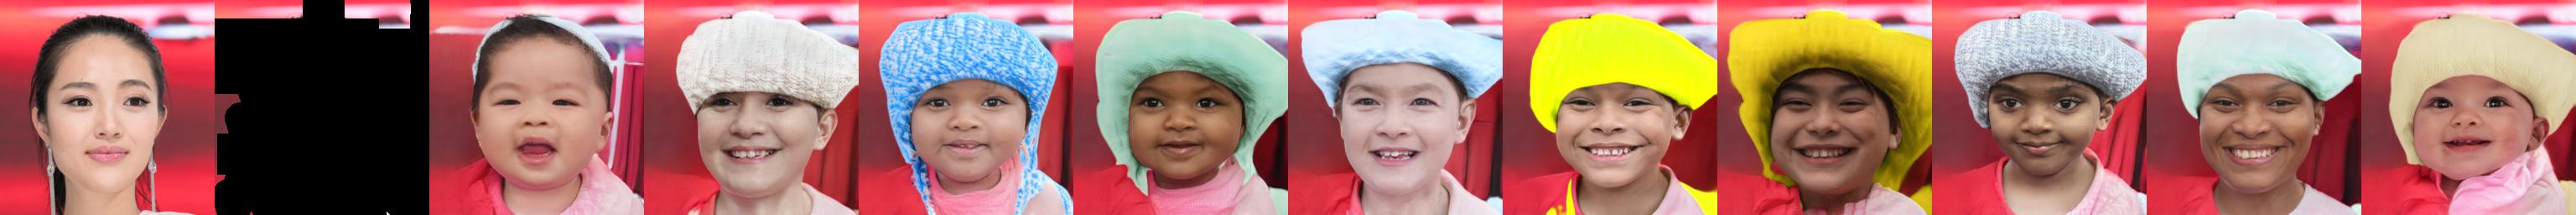
\includegraphics[trim=512px 0px 0px 0px, clip, height=\cmgfailureimgheight]{figs/cigcvae/co_mod_gan_failure/co_mod_gan_56_4_16.jpg}
    \caption{Sampled completions}
  \end{subfigure}
  \begin{subfigure}[t]{0.1\textwidth}
    \centering
    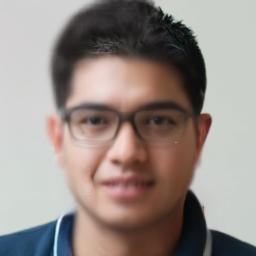
\includegraphics[height=\cmgfailureimgheight]{figs/cigcvae/co_mod_gan_failure/avg_co_mod_gan_0_3_2.jpg}
    %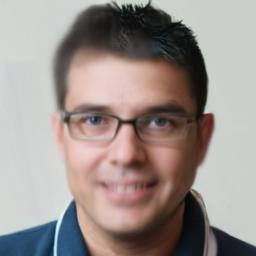
\includegraphics[height=\cmgfailureimgheight]{figs/cigcvae/co_mod_gan_failure/avg_co_mod_gan_0_3_6.jpg}
    %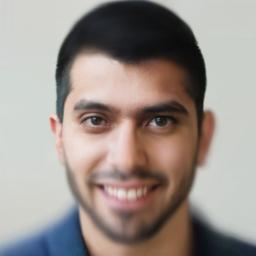
\includegraphics[height=\cmgfailureimgheight]{figs/cigcvae/co_mod_gan_failure/avg_co_mod_gan_0_3_7.jpg}
    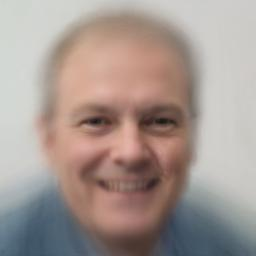
\includegraphics[height=\cmgfailureimgheight]{figs/cigcvae/co_mod_gan_failure/avg_co_mod_gan_0_4_2.jpg}
    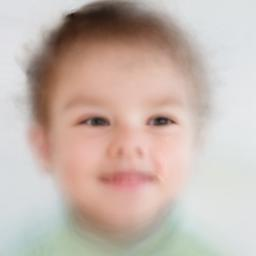
\includegraphics[height=\cmgfailureimgheight]{figs/cigcvae/co_mod_gan_failure/avg_co_mod_gan_1_4_2.jpg}
    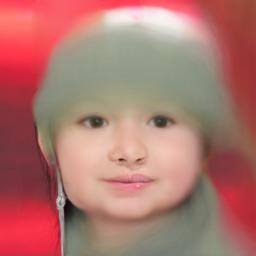
\includegraphics[height=\cmgfailureimgheight]{figs/cigcvae/co_mod_gan_failure/avg_co_mod_gan_56_4_12.jpg}
    %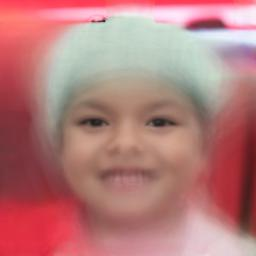
\includegraphics[height=\cmgfailureimgheight]{figs/cigcvae/co_mod_gan_failure/avg_co_mod_gan_56_4_16.jpg}
    \caption{Mean}
  \end{subfigure}
  %%%%%%%%%%%%%%%%%%%%%%
  \caption{Examples of completions lacking semantic diversity in CoModGAN. Panel
    (a) shows the true image and the masked version on which the completions are
    conditioned. Panel (b) shows 10 completions sampled randomly from the
    CoModGAN model. Panel (c) shows the mean image computed from 100 sampled
    completions. On each row, the completions are mostly semantically similar to
    eachother yet different from the ground truth image, indicating that they
    are not faithfully representing the true posterior. This behaviour can be
    contrasted with that of IPA in \cref{fig:cigcvae-comodgan-failure-aipo}.}
  \label{fig:cigcvae-comodgan-failure}
  \vspace{.5cm}
  \begin{subfigure}[t]{0.14\textwidth}
    \centering
    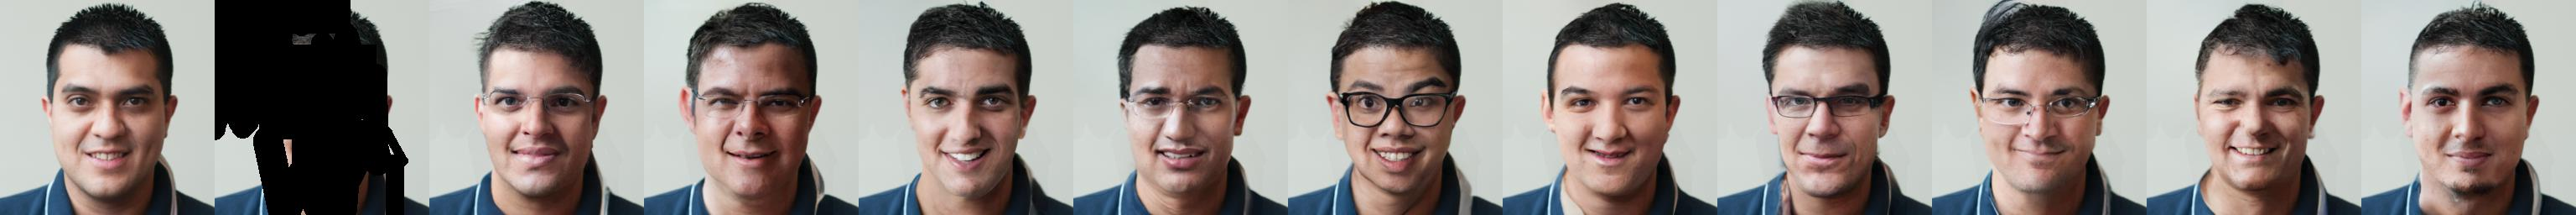
\includegraphics[trim=0px 0px 2560px 0px, clip, height=\cmgfailureimgheight]{figs/cigcvae/co_mod_gan_failure/aipo_0_3_2.jpg}
    %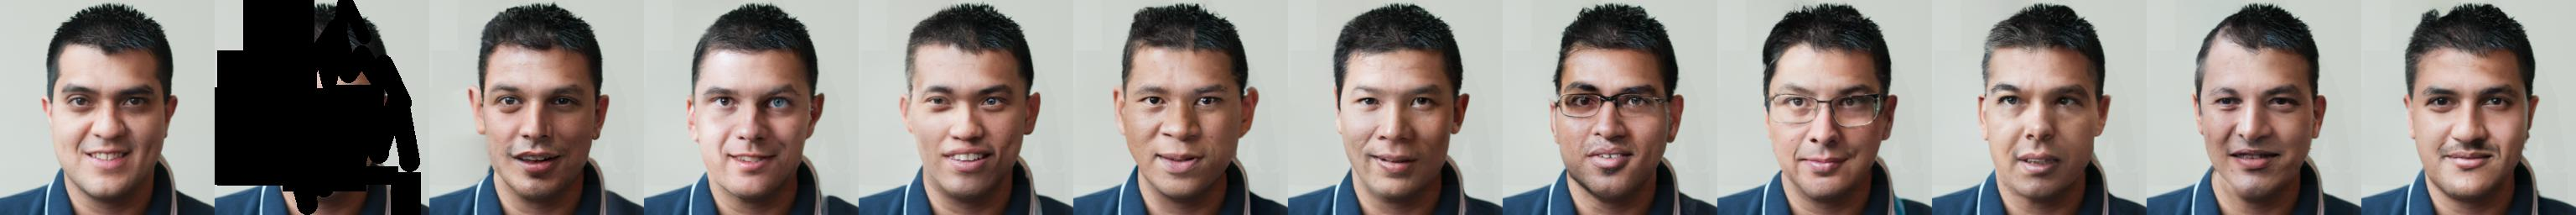
\includegraphics[trim=0px 0px 2560px 0px, clip, height=\cmgfailureimgheight]{figs/cigcvae/co_mod_gan_failure/aipo_0_3_6.jpg}
    %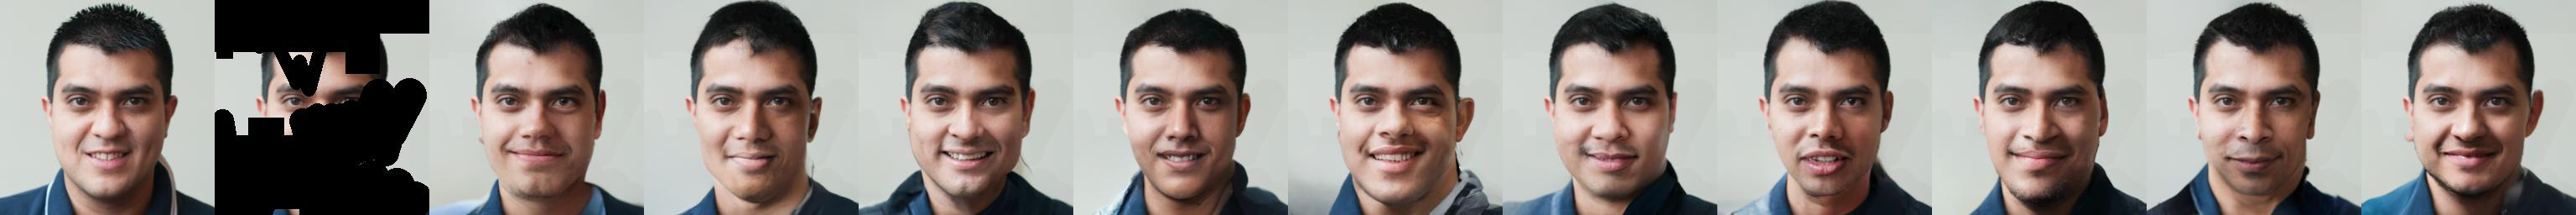
\includegraphics[trim=0px 0px 2560px 0px, clip, height=\cmgfailureimgheight]{figs/cigcvae/co_mod_gan_failure/aipo_0_3_7.jpg}
    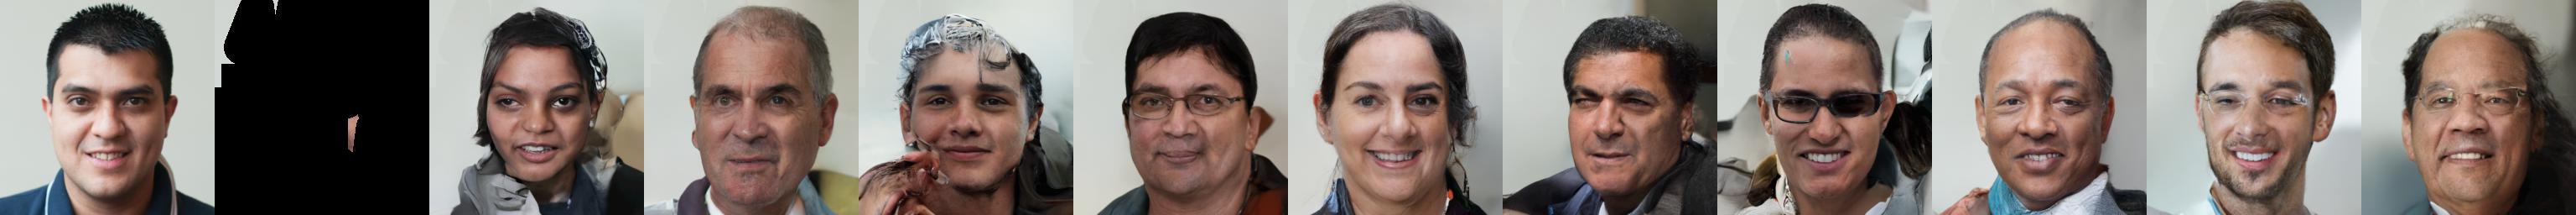
\includegraphics[trim=0px 0px 2560px 0px, clip, height=\cmgfailureimgheight]{figs/cigcvae/co_mod_gan_failure/aipo_0_4_2.jpg}
    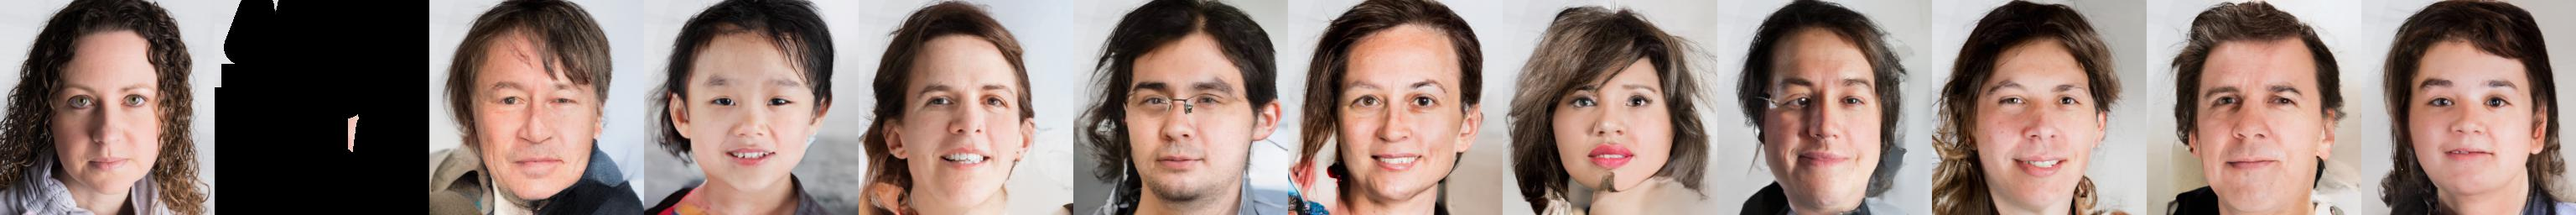
\includegraphics[trim=0px 0px 2560px 0px, clip, height=\cmgfailureimgheight]{figs/cigcvae/co_mod_gan_failure/aipo_1_4_2.jpg}
    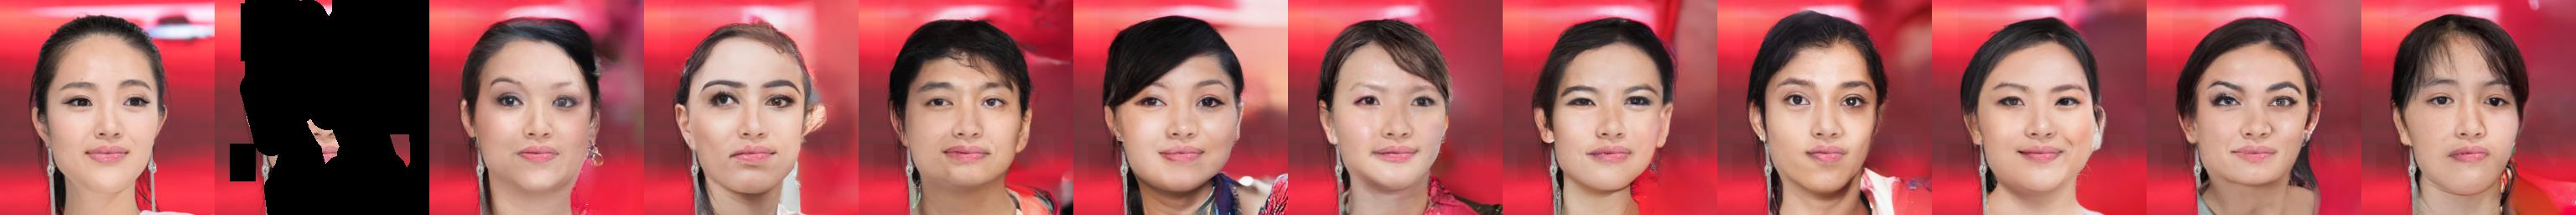
\includegraphics[trim=0px 0px 2560px 0px, clip, height=\cmgfailureimgheight]{figs/cigcvae/co_mod_gan_failure/aipo_56_4_12.jpg}
    %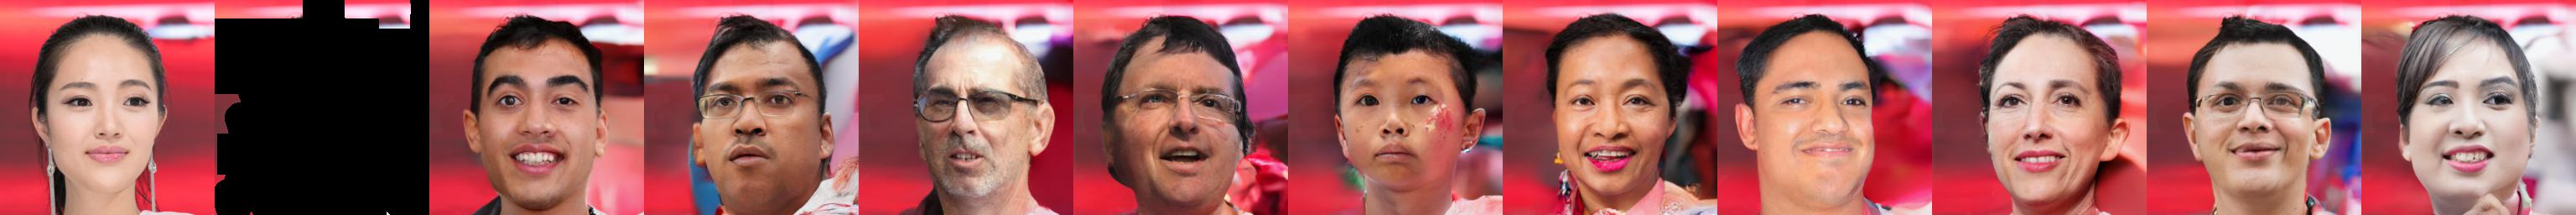
\includegraphics[trim=0px 0px 2560px 0px, clip, height=\cmgfailureimgheight]{figs/cigcvae/co_mod_gan_failure/aipo_56_4_16.jpg}
    \caption{$\I, \partI$}
  \end{subfigure}
  \begin{subfigure}[t]{0.73\textwidth}
    \centering
    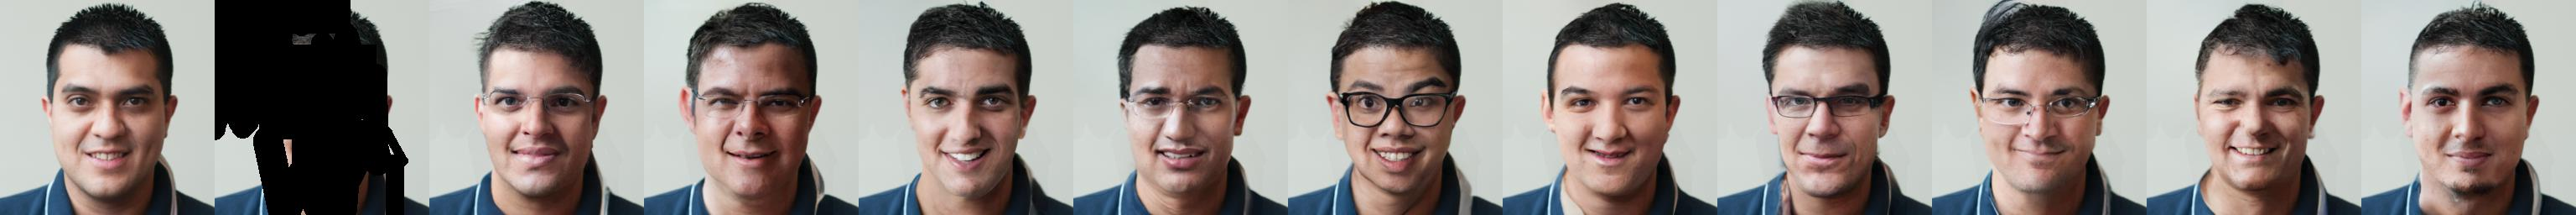
\includegraphics[trim=512px 0px 0px 0px, clip, height=\cmgfailureimgheight]{figs/cigcvae/co_mod_gan_failure/aipo_0_3_2.jpg}
    %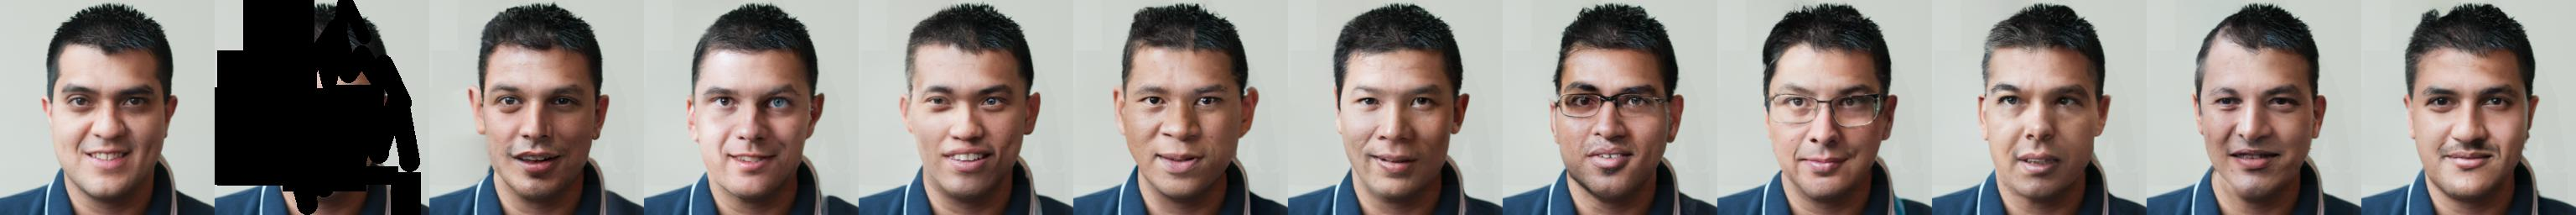
\includegraphics[trim=512px 0px 0px 0px, clip, height=\cmgfailureimgheight]{figs/cigcvae/co_mod_gan_failure/aipo_0_3_6.jpg}
    %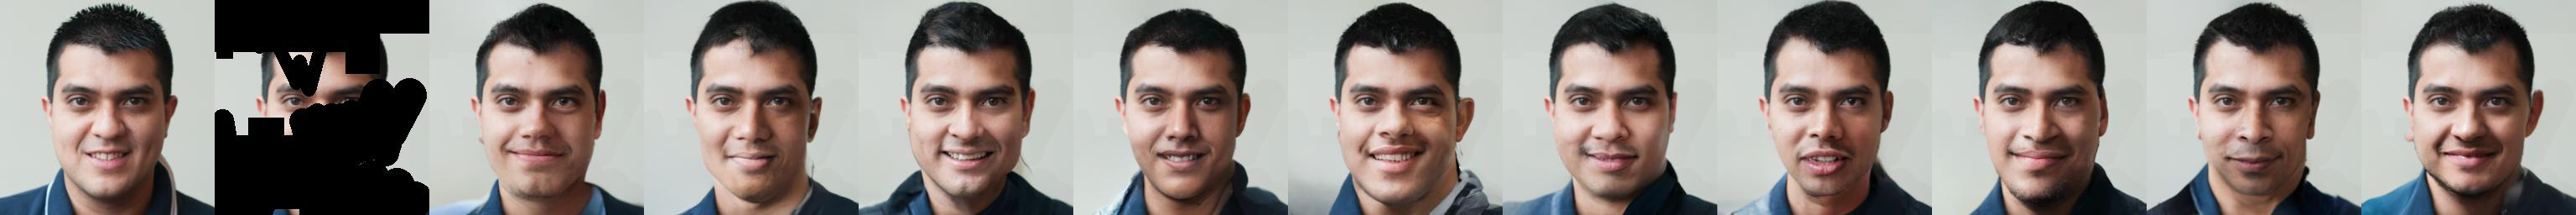
\includegraphics[trim=512px 0px 0px 0px, clip, height=\cmgfailureimgheight]{figs/cigcvae/co_mod_gan_failure/aipo_0_3_7.jpg}
    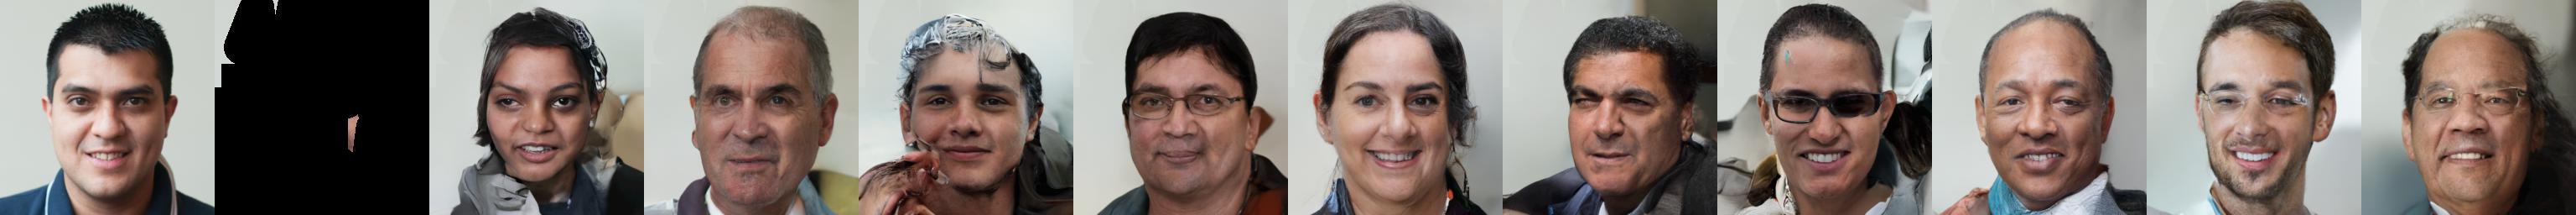
\includegraphics[trim=512px 0px 0px 0px, clip, height=\cmgfailureimgheight]{figs/cigcvae/co_mod_gan_failure/aipo_0_4_2.jpg}
    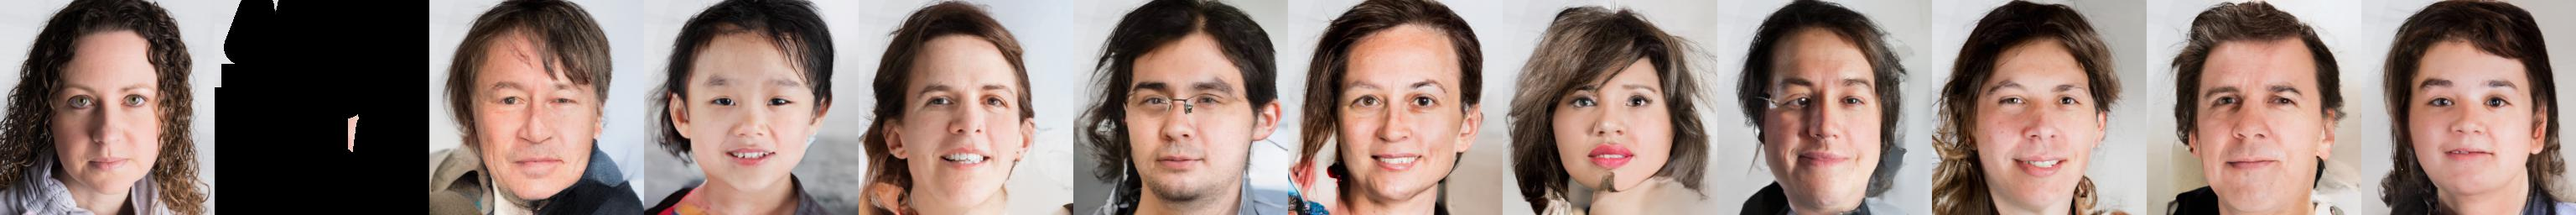
\includegraphics[trim=512px 0px 0px 0px, clip, height=\cmgfailureimgheight]{figs/cigcvae/co_mod_gan_failure/aipo_1_4_2.jpg}
    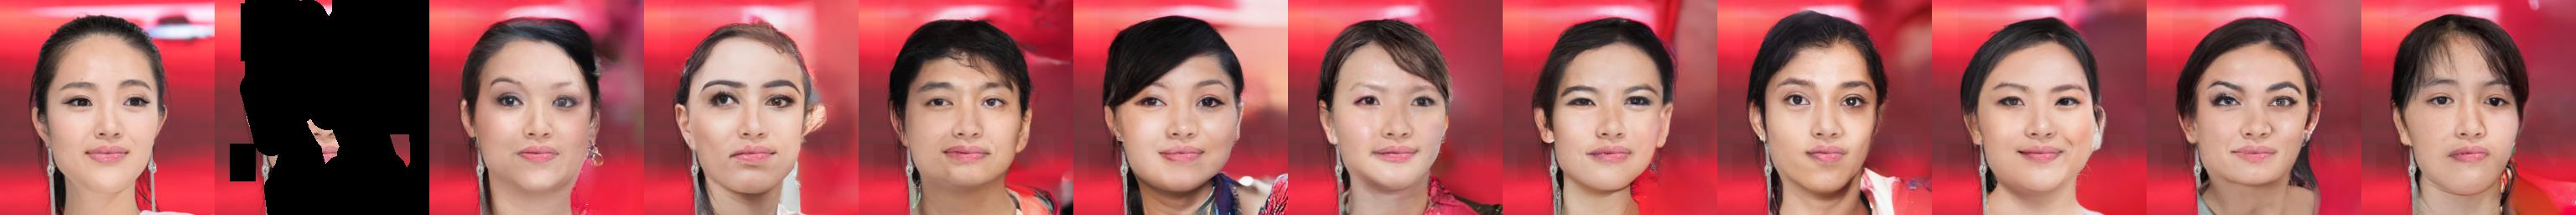
\includegraphics[trim=512px 0px 0px 0px, clip, height=\cmgfailureimgheight]{figs/cigcvae/co_mod_gan_failure/aipo_56_4_12.jpg}
    %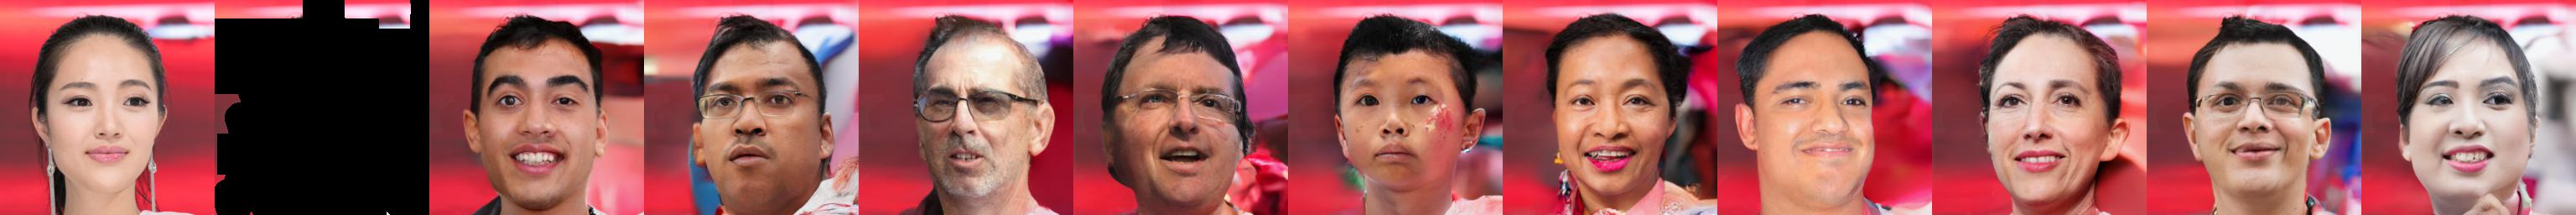
\includegraphics[trim=512px 0px 0px 0px, clip, height=\cmgfailureimgheight]{figs/cigcvae/co_mod_gan_failure/aipo_56_4_16.jpg}
    \caption{Sampled completions}
  \end{subfigure}
  \begin{subfigure}[t]{0.1\textwidth}
    \centering
    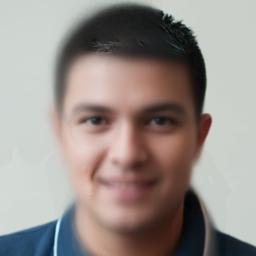
\includegraphics[height=\cmgfailureimgheight]{figs/cigcvae/co_mod_gan_failure/avg_aipo_0_3_2.jpg}
    %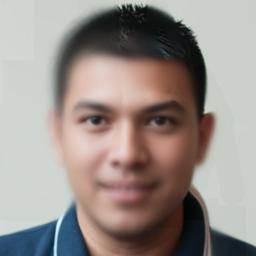
\includegraphics[height=\cmgfailureimgheight]{figs/cigcvae/co_mod_gan_failure/avg_aipo_0_3_6.jpg}
    %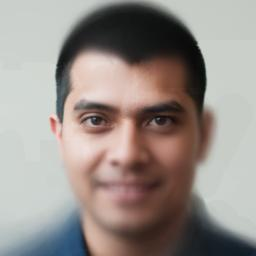
\includegraphics[height=\cmgfailureimgheight]{figs/cigcvae/co_mod_gan_failure/avg_aipo_0_3_7.jpg}
    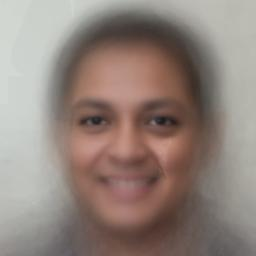
\includegraphics[height=\cmgfailureimgheight]{figs/cigcvae/co_mod_gan_failure/avg_aipo_0_4_2.jpg}
    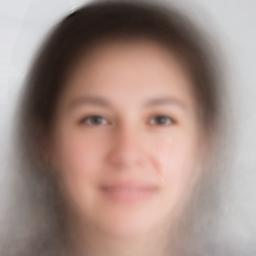
\includegraphics[height=\cmgfailureimgheight]{figs/cigcvae/co_mod_gan_failure/avg_aipo_1_4_2.jpg}
    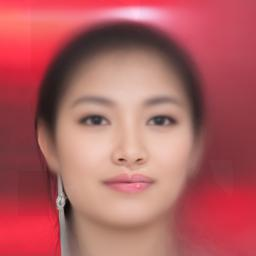
\includegraphics[height=\cmgfailureimgheight]{figs/cigcvae/co_mod_gan_failure/avg_aipo_56_4_12.jpg}
    %\includegraphics[height=\cmgfailureimgheight]{figs/cigcvae/co_mod_gan_failure/avg_aipo_56_4_16.jpg}
    \caption{Mean}
  \end{subfigure}
  %%%%%%%%%%%%%%%%%%%%%%
  \caption{Examples completions from our IPA model, to compare with
    \cref{fig:cigcvae-comodgan-failure}. These samples from IPA provide a much better
    representation of the inherent uncertainty in the image given the
    observations. We did not find any $(\I{}, \partI{})$ pairs on which the IPA
    model failed in the same way as CoModGAN in \cref{fig:cigcvae-comodgan-failure}. }
  \label{fig:cigcvae-comodgan-failure-aipo}
\end{figure*}

\section{Image samples}\label{supp:cigcvae-image-samples}


\Cref{fig:cigcvae-cifar-samples-0,fig:cigcvae-imagenet-samples,fig:cigcvae-ffhq-samples,fig:cigcvae-bags-samples,fig:cigcvae-shoes-samples,fig:cigcvae-xray-samples}
on the following pages show conditionally generated images for all datasets we have
experimented with, from both IPA and our baselines. It is apparent from the
image samples, particularly when the number of observed pixels is small, that
IPA-R has less sample diversity than IPA, which can be explained by the
mode-seeking behaviour of the reverse-KL and subsequent under-estimation of
posterior uncertainty \citep{minka2005divergence}. Finally, we note a flaw with
some of the completions produced by IPA: a lack of bilateral symmetry in
FFHQ-256 samples. Again, this is most apparent when few pixels are observed.
This issue can be seen in unconditional samples from the underlying VAEs as well
(see the samples reported by \citet{child2020very}). Therefore, it is likely
that any future advances in image modelling with VAEs could be integrated to
improve this aspect of the results.

\newcommand{\qualimgheight}{4cm} 
\newcommand{\qualcaption}[1]{Sampled
  completions from each method for #1 image. Panels (a), (d) and (h) all show
  the true image and the masked image on which the samples in each row are
  conditioned. Panels (b) and (c) show completions from IPA and IPA-R. (g) and
  (k) show the single deterministic completion produced by CE and RFR
  respectively. Each of the remaining panels show five completions for the
  stochastic baselines.} \newcommand{\freeformimgheight}{0.8cm}


% CIFAR samples -------------------------------------------------------------------------------------------------------------
\newcommand{\cifarimgheight}{1.2cm}
\newcommand{\clipby}{20}
  \begin{figure*}[t]
    \centering
    \begin{subfigure}[t]{0.11\textwidth}
      \centering
      \includegraphics[height=\cifarimgheight]{figs/cigcvae/image-samples/cifar10/freeform_aipo_0_gt_masked}
      \includegraphics[height=\cifarimgheight]{figs/cigcvae/image-samples/cifar10/freeform_aipo_1_gt_masked}
      \includegraphics[height=\cifarimgheight]{figs/cigcvae/image-samples/cifar10/freeform_aipo_3_gt_masked}
      \caption{$\I, \partI$}
    \end{subfigure}
    \begin{subfigure}[t]{0.17\textwidth}
      \centering
      \includegraphics[height=\cifarimgheight]{figs/cigcvae/image-samples/cifar10/freeform_aipo_0_t=0.85_samples}
      \includegraphics[height=\cifarimgheight]{figs/cigcvae/image-samples/cifar10/freeform_aipo_1_t=0.85_samples}
      \includegraphics[height=\cifarimgheight]{figs/cigcvae/image-samples/cifar10/freeform_aipo_3_t=0.85_samples}
      \caption{IPA, $t=0.85$}
    \end{subfigure}
    \begin{subfigure}[t]{0.17\textwidth}
      \centering
      \includegraphics[height=\cifarimgheight]{figs/cigcvae/image-samples/cifar10/freeform_aipo_0_samples}
      \includegraphics[height=\cifarimgheight]{figs/cigcvae/image-samples/cifar10/freeform_aipo_1_samples}
      \includegraphics[height=\cifarimgheight]{figs/cigcvae/image-samples/cifar10/freeform_aipo_3_samples}
      \caption{IPA}
    \end{subfigure}
    \begin{subfigure}[t]{0.17\textwidth}
      \centering
      \includegraphics[height=\cifarimgheight]{figs/cigcvae/image-samples/cifar10/freeform_aipo_0_imagenet_samples}
      \includegraphics[height=\cifarimgheight]{figs/cigcvae/image-samples/cifar10/freeform_aipo_1_imagenet_samples}
      \includegraphics[height=\cifarimgheight]{figs/cigcvae/image-samples/cifar10/freeform_aipo_3_imagenet_samples}
      \caption{\scriptsize IPA from ImageNet}
    \end{subfigure}
    \begin{subfigure}[t]{0.17\textwidth}
      \centering
      \includegraphics[height=\cifarimgheight]{figs/cigcvae/image-samples/cifar10/freeform_aipo_0_scratch_samples}
      \includegraphics[height=\cifarimgheight]{figs/cigcvae/image-samples/cifar10/freeform_aipo_1_scratch_samples}
      \includegraphics[height=\cifarimgheight]{figs/cigcvae/image-samples/cifar10/freeform_aipo_3_scratch_samples}
      \caption{\scriptsize IPA from scratch}
    \end{subfigure}
    \begin{subfigure}[t]{0.17\textwidth}
      \centering
      \includegraphics[height=\cifarimgheight]{figs/cigcvae/image-samples/cifar10/freeform_aipo-r_0_samples}
      \includegraphics[height=\cifarimgheight]{figs/cigcvae/image-samples/cifar10/freeform_aipo-r_1_samples}
      \includegraphics[height=\cifarimgheight]{figs/cigcvae/image-samples/cifar10/freeform_aipo-r_3_samples}
      \caption{IPA-R}
    \end{subfigure}
    %%%%%%%%%%%%%%%%%%%%%%
    \begin{subfigure}[t]{0.11\textwidth}
      \centering
      \includegraphics[height=\cifarimgheight]{figs/cigcvae/image-samples/cifar10/freeform_aipo_0_gt_masked}
      \includegraphics[height=\cifarimgheight]{figs/cigcvae/image-samples/cifar10/freeform_aipo_1_gt_masked}
      \includegraphics[height=\cifarimgheight]{figs/cigcvae/image-samples/cifar10/freeform_aipo_3_gt_masked}
      \caption*{$\I, \partI$}
    \end{subfigure}
    \begin{subfigure}[t]{0.17\textwidth}
      \centering
      \includegraphics[height=\cifarimgheight]{figs/cigcvae/image-samples/cifar10/freeform_co_mod_gan_0_samples}
      \includegraphics[height=\cifarimgheight]{figs/cigcvae/image-samples/cifar10/freeform_co_mod_gan_1_samples}
      \includegraphics[height=\cifarimgheight]{figs/cigcvae/image-samples/cifar10/freeform_co_mod_gan_3_samples}
      \caption{CoModGAN}
    \end{subfigure}
    \begin{subfigure}[t]{0.17\textwidth}
      \centering
      \includegraphics[height=\cifarimgheight]{figs/cigcvae/image-samples/cifar10/freeform_pic_0_samples}
      \includegraphics[height=\cifarimgheight]{figs/cigcvae/image-samples/cifar10/freeform_pic_1_samples}
      \includegraphics[height=\cifarimgheight]{figs/cigcvae/image-samples/cifar10/freeform_pic_3_samples}
      \caption{PIC}
    \end{subfigure}
    \begin{subfigure}[t]{0.17\textwidth}
      \centering
      \includegraphics[height=\cifarimgheight]{figs/cigcvae/image-samples/cifar10/freeform_anp_0_samples}
      \includegraphics[height=\cifarimgheight]{figs/cigcvae/image-samples/cifar10/freeform_anp_1_samples}
      \includegraphics[height=\cifarimgheight]{figs/cigcvae/image-samples/cifar10/freeform_anp_3_samples}
      \caption{ANP}
    \end{subfigure}
    \begin{subfigure}[t]{0.17\textwidth}
      \centering
      \includegraphics[height=\cifarimgheight]{figs/cigcvae/image-samples/cifar10/freeform_vq_vae_0_samples}
      \includegraphics[height=\cifarimgheight]{figs/cigcvae/image-samples/cifar10/freeform_vq_vae_1_samples}
      \includegraphics[height=\cifarimgheight]{figs/cigcvae/image-samples/cifar10/freeform_vq_vae_3_samples}
      \caption{VQ-VAE}
    \end{subfigure}
    \begin{subfigure}[t]{0.08\textwidth}
      \centering
      \includegraphics[height=\cifarimgheight]{figs/cigcvae/image-samples/cifar10/freeform_ce_0_samples}
      \includegraphics[height=\cifarimgheight]{figs/cigcvae/image-samples/cifar10/freeform_ce_1_samples}
      \includegraphics[height=\cifarimgheight]{figs/cigcvae/image-samples/cifar10/freeform_ce_3_samples}
      \caption{CE}
    \end{subfigure}
    \begin{subfigure}[t]{0.08\textwidth}
      \centering
      \includegraphics[height=\cifarimgheight]{figs/cigcvae/image-samples/cifar10/freeform_rfr_0_samples}
      \includegraphics[height=\cifarimgheight]{figs/cigcvae/image-samples/cifar10/freeform_rfr_1_samples}
      \includegraphics[height=\cifarimgheight]{figs/cigcvae/image-samples/cifar10/freeform_rfr_3_samples}
      \caption{RFR}
    \end{subfigure}
    \caption{Sampled completions on CIFAR-10. Panel (a) shows test images along
      with masked versions on which samples in each row are conditioned. The
      remaining panels in the top row show samples from IPA (with an artifact
      pretrained on the same dataset) with and without a reduced temperature,
      IPA with an artifact pretrained on ImageNet, a conditional VAE trained
      from scratch, and finally IPA-R (with an artifact pretrained on the same
      dataset). The bottom row shows samples from our baselines. Three samples
      per masked image are shown for each stochastic method, while the single
      deterministic completion is shown for CE and RFR. All samples are taken
      with temperature 1 where not stated otherwise.}
    \label{fig:cigcvae-cifar-samples-0}
  \end{figure*}


  % ImageNet64 samples -------------------------------------------------------------------------------------------------------
% show samples for 0, 1, 2, 3, 4
\newcommand{\imagenetimgheight}{0.8cm}
  \begin{figure*}[t]
    \centering
    \begin{subfigure}[t]{0.15\textwidth}
      \centering
      \includegraphics[height=\imagenetimgheight]{figs/cigcvae/image-samples/imagenet64/freeform_aipo_0_gt_masked.png}
      \includegraphics[height=\imagenetimgheight]{figs/cigcvae/image-samples/imagenet64/freeform_aipo_1_gt_masked.png}
      \includegraphics[height=\imagenetimgheight]{figs/cigcvae/image-samples/imagenet64/freeform_aipo_2_gt_masked.png}
      \includegraphics[height=\imagenetimgheight]{figs/cigcvae/image-samples/imagenet64/freeform_aipo_3_gt_masked.png}
      \includegraphics[height=\imagenetimgheight]{figs/cigcvae/image-samples/imagenet64/freeform_aipo_4_gt_masked.png}
      \caption{$\I, \partI$}
    \end{subfigure}
    \begin{subfigure}[t]{0.2\textwidth}
      \centering
      \includegraphics[height=\imagenetimgheight]{figs/cigcvae/image-samples/imagenet64/freeform_aipo_0_t=0.85_samples.png}
      \includegraphics[height=\imagenetimgheight]{figs/cigcvae/image-samples/imagenet64/freeform_aipo_1_t=0.85_samples.png}
      \includegraphics[height=\imagenetimgheight]{figs/cigcvae/image-samples/imagenet64/freeform_aipo_2_t=0.85_samples.png}
      \includegraphics[height=\imagenetimgheight]{figs/cigcvae/image-samples/imagenet64/freeform_aipo_3_t=0.85_samples.png}
      \includegraphics[height=\imagenetimgheight]{figs/cigcvae/image-samples/imagenet64/freeform_aipo_4_t=0.85_samples.png}
      \caption{IPA, $t=0.85$}
    \end{subfigure}
    \begin{subfigure}[t]{0.2\textwidth}
      \centering
      \includegraphics[height=\imagenetimgheight]{figs/cigcvae/image-samples/imagenet64/freeform_aipo_0_samples.png}
      \includegraphics[height=\imagenetimgheight]{figs/cigcvae/image-samples/imagenet64/freeform_aipo_1_samples.png}
      \includegraphics[height=\imagenetimgheight]{figs/cigcvae/image-samples/imagenet64/freeform_aipo_2_samples.png}
      \includegraphics[height=\imagenetimgheight]{figs/cigcvae/image-samples/imagenet64/freeform_aipo_3_samples.png}
      \includegraphics[height=\imagenetimgheight]{figs/cigcvae/image-samples/imagenet64/freeform_aipo_4_samples.png}
      \caption{IPA}
    \end{subfigure}
    \begin{subfigure}[t]{0.2\textwidth}
      \centering
      \includegraphics[height=\imagenetimgheight]{figs/cigcvae/image-samples/imagenet64/freeform_aipo_0_scratch_samples.png}
      \includegraphics[height=\imagenetimgheight]{figs/cigcvae/image-samples/imagenet64/freeform_aipo_1_scratch_samples.png}
      \includegraphics[height=\imagenetimgheight]{figs/cigcvae/image-samples/imagenet64/freeform_aipo_2_scratch_samples.png}
      \includegraphics[height=\imagenetimgheight]{figs/cigcvae/image-samples/imagenet64/freeform_aipo_3_scratch_samples.png}
      \includegraphics[height=\imagenetimgheight]{figs/cigcvae/image-samples/imagenet64/freeform_aipo_4_scratch_samples.png}
      \caption{IPA from scratch}
    \end{subfigure}
    \begin{subfigure}[t]{0.2\textwidth}
      \centering
      \includegraphics[height=\imagenetimgheight]{figs/cigcvae/image-samples/imagenet64/freeform_aipo-r_0_samples.png}
      \includegraphics[height=\imagenetimgheight]{figs/cigcvae/image-samples/imagenet64/freeform_aipo-r_1_samples.png}
      \includegraphics[height=\imagenetimgheight]{figs/cigcvae/image-samples/imagenet64/freeform_aipo-r_2_samples.png}
      \includegraphics[height=\imagenetimgheight]{figs/cigcvae/image-samples/imagenet64/freeform_aipo-r_3_samples.png}
      \includegraphics[height=\imagenetimgheight]{figs/cigcvae/image-samples/imagenet64/freeform_aipo-r_4_samples.png}
      \caption{IPA-R}
    \end{subfigure}
    \begin{subfigure}[t]{0.15\textwidth}
      \centering
      \includegraphics[height=\imagenetimgheight]{figs/cigcvae/image-samples/imagenet64/freeform_aipo_0_gt_masked.png}
      \includegraphics[height=\imagenetimgheight]{figs/cigcvae/image-samples/imagenet64/freeform_aipo_1_gt_masked.png}
      \includegraphics[height=\imagenetimgheight]{figs/cigcvae/image-samples/imagenet64/freeform_aipo_2_gt_masked.png}
      \includegraphics[height=\imagenetimgheight]{figs/cigcvae/image-samples/imagenet64/freeform_aipo_3_gt_masked.png}
      \includegraphics[height=\imagenetimgheight]{figs/cigcvae/image-samples/imagenet64/freeform_aipo_4_gt_masked.png}
      \caption*{$\I, \partI$}
    \end{subfigure}
    \begin{subfigure}[t]{0.2\textwidth}
      \centering
      \includegraphics[height=\imagenetimgheight]{figs/cigcvae/image-samples/imagenet64/freeform_co_mod_gan_0_samples.png}
      \includegraphics[height=\imagenetimgheight]{figs/cigcvae/image-samples/imagenet64/freeform_co_mod_gan_1_samples.png}
      \includegraphics[height=\imagenetimgheight]{figs/cigcvae/image-samples/imagenet64/freeform_co_mod_gan_2_samples.png}
      \includegraphics[height=\imagenetimgheight]{figs/cigcvae/image-samples/imagenet64/freeform_co_mod_gan_3_samples.png}
      \includegraphics[height=\imagenetimgheight]{figs/cigcvae/image-samples/imagenet64/freeform_co_mod_gan_4_samples.png}
      \caption{CoModGAN}
    \end{subfigure}
    \begin{subfigure}[t]{0.2\textwidth}
      \centering
      \includegraphics[height=\imagenetimgheight]{figs/cigcvae/image-samples/imagenet64/freeform_pic_0_samples.png}
      \includegraphics[height=\imagenetimgheight]{figs/cigcvae/image-samples/imagenet64/freeform_pic_1_samples.png}
      \includegraphics[height=\imagenetimgheight]{figs/cigcvae/image-samples/imagenet64/freeform_pic_2_samples.png}
      \includegraphics[height=\imagenetimgheight]{figs/cigcvae/image-samples/imagenet64/freeform_pic_3_samples.png}
      \includegraphics[height=\imagenetimgheight]{figs/cigcvae/image-samples/imagenet64/freeform_pic_4_samples.png}
      \caption{PIC}
    \end{subfigure}
    \begin{subfigure}[t]{0.4\textwidth}
      \setlength{\fboxrule}{0pt}
      \fbox{
        \begin{minipage}{5cm}
          \hfill\hspace{5cm}
        \end{minipage}
      }
    \end{subfigure}
    \caption{Sampled completions on ImageNet-64. Panel (a) shows a test image
      and the masked version on which samples in each row are conditioned. The
      remaining panels in the top row show samples from IPA with and without a
      reduced temperature, from an IPA-style conditional VAE trained from
      scratch, and from IPA-R. The bottom row shows samples CoModGAN.}
    \vspace{-.5cm}
    \label{fig:cigcvae-imagenet-samples}
  \end{figure*}


  % FFHQ samples -------------------------------------------------------------------------------------------------------------
% show samples for 0, 13, 32
\newcommand{\ffhqimgheight}{0.8cm}
  \begin{figure*}[t]
    \centering
    \begin{subfigure}[t]{0.22\textwidth}
      \centering
      \includegraphics[height=\ffhqimgheight]{figs/cigcvae/image-samples/ffhq256/freeform_aipo_0_gt_masked.jpg}
      \includegraphics[height=\ffhqimgheight]{figs/cigcvae/image-samples/ffhq256/freeform_aipo_13_gt_masked.jpg}
      \includegraphics[height=\ffhqimgheight]{figs/cigcvae/image-samples/ffhq256/freeform_aipo_32_gt_masked.jpg}
      \caption{$\I, \partI$}
    \end{subfigure}
    \begin{subfigure}[t]{0.25\textwidth}
      \centering
      \includegraphics[height=\ffhqimgheight]{figs/cigcvae/image-samples/ffhq256/freeform_aipo_0_t=0.85_samples.jpg}
      \includegraphics[height=\ffhqimgheight]{figs/cigcvae/image-samples/ffhq256/freeform_aipo_13_t=0.85_samples.jpg}
      \includegraphics[height=\ffhqimgheight]{figs/cigcvae/image-samples/ffhq256/freeform_aipo_32_t=0.85_samples.jpg}
      \caption{IPA, $t=0.85$}
    \end{subfigure}
    \begin{subfigure}[t]{0.25\textwidth}
      \centering
      \includegraphics[height=\ffhqimgheight]{figs/cigcvae/image-samples/ffhq256/freeform_aipo_0_samples.jpg}
      \includegraphics[height=\ffhqimgheight]{figs/cigcvae/image-samples/ffhq256/freeform_aipo_13_samples.jpg}
      \includegraphics[height=\ffhqimgheight]{figs/cigcvae/image-samples/ffhq256/freeform_aipo_32_samples.jpg}
      \caption{IPA}
    \end{subfigure}
    \begin{subfigure}[t]{0.25\textwidth}
      \centering
      \includegraphics[height=\ffhqimgheight]{figs/cigcvae/image-samples/ffhq256/freeform_aipo-r_0_samples.jpg}
      \includegraphics[height=\ffhqimgheight]{figs/cigcvae/image-samples/ffhq256/freeform_aipo-r_13_samples.jpg}
      \includegraphics[height=\ffhqimgheight]{figs/cigcvae/image-samples/ffhq256/freeform_aipo-r_32_samples.jpg}
      \caption{IPA-R}
    \end{subfigure}
    %%%%%%%%%%%%%%%%%%%%%%
    \begin{subfigure}[t]{0.22\textwidth}
      \centering
      \includegraphics[height=\ffhqimgheight]{figs/cigcvae/image-samples/ffhq256/freeform_aipo_0_gt_masked.jpg}
      \includegraphics[height=\ffhqimgheight]{figs/cigcvae/image-samples/ffhq256/freeform_aipo_13_gt_masked.jpg}
      \includegraphics[height=\ffhqimgheight]{figs/cigcvae/image-samples/ffhq256/freeform_aipo_32_gt_masked.jpg}
      \caption*{$\I, \partI$}
    \end{subfigure}
    \begin{subfigure}[t]{0.25\textwidth}
      \centering
      \includegraphics[height=\ffhqimgheight]{figs/cigcvae/image-samples/ffhq256/freeform_co_mod_gan_0_samples.jpg}
      \includegraphics[height=\ffhqimgheight]{figs/cigcvae/image-samples/ffhq256/freeform_co_mod_gan_13_samples.jpg}
      \includegraphics[height=\ffhqimgheight]{figs/cigcvae/image-samples/ffhq256/freeform_co_mod_gan_32_samples.jpg}
      \caption{CoModGAN}
    \end{subfigure}
    \begin{subfigure}[t]{0.25\textwidth}
      \centering
      \includegraphics[height=\ffhqimgheight]{figs/cigcvae/image-samples/ffhq256/freeform_pic_0_samples.jpg}
      \includegraphics[height=\ffhqimgheight]{figs/cigcvae/image-samples/ffhq256/freeform_pic_13_samples.jpg}
      \includegraphics[height=\ffhqimgheight]{figs/cigcvae/image-samples/ffhq256/freeform_pic_32_samples.jpg}
      \caption{PIC}
    \end{subfigure}
    \begin{subfigure}[t]{0.25\textwidth}
      \centering
      \includegraphics[height=\ffhqimgheight]{figs/cigcvae/image-samples/ffhq256/freeform_anp_0_samples.jpg}
      \includegraphics[height=\ffhqimgheight]{figs/cigcvae/image-samples/ffhq256/freeform_anp_13_samples.jpg}
      \includegraphics[height=\ffhqimgheight]{figs/cigcvae/image-samples/ffhq256/freeform_anp_32_samples.jpg}
      \caption{ANP}
    \end{subfigure}
    %%%%%%%%%%%%%%%%%%%%%%
    \begin{subfigure}[t]{0.22\textwidth}
      \centering
      \includegraphics[height=\ffhqimgheight]{figs/cigcvae/image-samples/ffhq256/freeform_aipo_0_gt_masked.jpg}
      \includegraphics[height=\ffhqimgheight]{figs/cigcvae/image-samples/ffhq256/freeform_aipo_13_gt_masked.jpg}
      \includegraphics[height=\ffhqimgheight]{figs/cigcvae/image-samples/ffhq256/freeform_aipo_32_gt_masked.jpg}
      \caption*{$\I, \partI$}
    \end{subfigure}
    \begin{subfigure}[t]{0.25\textwidth}
      \centering
      \includegraphics[height=\ffhqimgheight]{figs/cigcvae/image-samples/ffhq256/freeform_vq_vae_0_samples.jpg}
      \includegraphics[height=\ffhqimgheight]{figs/cigcvae/image-samples/ffhq256/freeform_vq_vae_13_samples.jpg}
      \includegraphics[height=\ffhqimgheight]{figs/cigcvae/image-samples/ffhq256/freeform_vq_vae_32_samples.jpg}
      \caption{VQ-VAE}
    \end{subfigure}
    \begin{subfigure}[t]{0.25\textwidth}
      \centering
      \includegraphics[height=\ffhqimgheight]{figs/cigcvae/image-samples/ffhq256/freeform_ce_0_samples.jpg}\\
      \includegraphics[height=\ffhqimgheight]{figs/cigcvae/image-samples/ffhq256/freeform_ce_13_samples.jpg}\\
      \includegraphics[height=\ffhqimgheight]{figs/cigcvae/image-samples/ffhq256/freeform_ce_32_samples.jpg}
      \caption{CE}
    \end{subfigure}
    \begin{subfigure}[t]{0.25\textwidth}
      \centering
      \includegraphics[height=\ffhqimgheight]{figs/cigcvae/image-samples/ffhq256/freeform_rfr_0_samples.jpg}\\
      \includegraphics[height=\ffhqimgheight]{figs/cigcvae/image-samples/ffhq256/freeform_rfr_13_samples.jpg}\\
      \includegraphics[height=\ffhqimgheight]{figs/cigcvae/image-samples/ffhq256/freeform_rfr_32_samples.jpg}
      \caption{RFR}
    \end{subfigure}
    \begin{subfigure}[t]{0.16\textwidth}
      \setlength{\fboxrule}{0pt}
      \fbox{
        \begin{minipage}{1in}
          \hfill\hspace{1in}
        \end{minipage}
      }
    \end{subfigure}
    \vspace{-.5cm}
    \caption{Sampled completions on FFHQ-256. Panel (a) shows test images along with
      masked versions on which samples in each row are conditioned. The
      remaining panels in the top row show samples from IPA with and without a
      reduced temperature and from IPA-R. The other rows show samples from our
      baselines. Four samples per masked image are shown for each stochastic
      method, while the single deterministic completion is shown for CE and
      RFR.}
    \vspace{-.5cm}
    \label{fig:cigcvae-ffhq-samples}
  \end{figure*}


  \clearpage
  % Edges2Stuff samples ------------------------------------------------------------------------------------------------------
% show samples for ...
\newcommand{\edgesstuffimgheight}{0.8cm}
  \begin{figure*}[t]
    \centering
    \begin{subfigure}[t]{0.15\textwidth}
      \centering
      \includegraphics[height=\edgesstuffimgheight]{figs/cigcvae/image-samples/bags/image_aipo_0_imagenet_gt_masked.png}
      \includegraphics[height=\edgesstuffimgheight]{figs/cigcvae/image-samples/bags/image_aipo_1_imagenet_gt_masked.png}
      \includegraphics[height=\edgesstuffimgheight]{figs/cigcvae/image-samples/bags/image_aipo_2_imagenet_gt_masked.png}
      \includegraphics[height=\edgesstuffimgheight]{figs/cigcvae/image-samples/bags/image_aipo_3_imagenet_gt_masked.png}
      \includegraphics[height=\edgesstuffimgheight]{figs/cigcvae/image-samples/bags/image_aipo_4_imagenet_gt_masked.png}
      \caption{$\I, \partI$}
    \end{subfigure}
    \begin{subfigure}[t]{0.27\textwidth}
      \centering
      \includegraphics[height=\edgesstuffimgheight]{figs/cigcvae/image-samples/bags/image_aipo_0_t=0.85_imagenet_samples.png}
      \includegraphics[height=\edgesstuffimgheight]{figs/cigcvae/image-samples/bags/image_aipo_1_t=0.85_imagenet_samples.png}
      \includegraphics[height=\edgesstuffimgheight]{figs/cigcvae/image-samples/bags/image_aipo_2_t=0.85_imagenet_samples.png}
      \includegraphics[height=\edgesstuffimgheight]{figs/cigcvae/image-samples/bags/image_aipo_3_t=0.85_imagenet_samples.png}
      \includegraphics[height=\edgesstuffimgheight]{figs/cigcvae/image-samples/bags/image_aipo_4_t=0.85_imagenet_samples.png}
      \caption{\scriptsize IPA from ImageNet, $t$=$0.85$}
    \end{subfigure}
    \begin{subfigure}[t]{0.27\textwidth}
      \centering
      \includegraphics[height=\edgesstuffimgheight]{figs/cigcvae/image-samples/bags/image_aipo_0_imagenet_samples.png}
      \includegraphics[height=\edgesstuffimgheight]{figs/cigcvae/image-samples/bags/image_aipo_1_imagenet_samples.png}
      \includegraphics[height=\edgesstuffimgheight]{figs/cigcvae/image-samples/bags/image_aipo_2_imagenet_samples.png}
      \includegraphics[height=\edgesstuffimgheight]{figs/cigcvae/image-samples/bags/image_aipo_3_imagenet_samples.png}
      \includegraphics[height=\edgesstuffimgheight]{figs/cigcvae/image-samples/bags/image_aipo_4_imagenet_samples.png}
      \caption{IPA from ImageNet}
    \end{subfigure}
    \begin{subfigure}[t]{0.27\textwidth}
      \centering
      \includegraphics[height=\edgesstuffimgheight]{figs/cigcvae/image-samples/bags/image_aipo_0_scratch_samples.png}
      \includegraphics[height=\edgesstuffimgheight]{figs/cigcvae/image-samples/bags/image_aipo_1_scratch_samples.png}
      \includegraphics[height=\edgesstuffimgheight]{figs/cigcvae/image-samples/bags/image_aipo_2_scratch_samples.png}
      \includegraphics[height=\edgesstuffimgheight]{figs/cigcvae/image-samples/bags/image_aipo_3_scratch_samples.png}
      \includegraphics[height=\edgesstuffimgheight]{figs/cigcvae/image-samples/bags/image_aipo_4_scratch_samples.png}
      \caption{IPA from scratch}
    \end{subfigure}
    \caption{Comparison of conditional generations on Edges2Bags.}
    \vspace{-.5cm}
    \label{fig:cigcvae-bags-samples}
  \end{figure*}

  \begin{figure*}[t]
    \centering
    \begin{subfigure}[t]{0.2\textwidth}
      \centering
      \includegraphics[height=\edgesstuffimgheight]{figs/cigcvae/image-samples/shoes/image_aipo_0_imagenet_gt_masked.png}
      \includegraphics[height=\edgesstuffimgheight]{figs/cigcvae/image-samples/shoes/image_aipo_1_imagenet_gt_masked.png}
      \includegraphics[height=\edgesstuffimgheight]{figs/cigcvae/image-samples/shoes/image_aipo_2_imagenet_gt_masked.png}
      \includegraphics[height=\edgesstuffimgheight]{figs/cigcvae/image-samples/shoes/image_aipo_3_imagenet_gt_masked.png}
      \includegraphics[height=\edgesstuffimgheight]{figs/cigcvae/image-samples/shoes/image_aipo_4_imagenet_gt_masked.png}
      \caption{$\I, \partI$}
    \end{subfigure}
    \begin{subfigure}[t]{0.25\textwidth}
      \centering
      \includegraphics[height=\edgesstuffimgheight]{figs/cigcvae/image-samples/shoes/image_aipo_0_t=0.85_imagenet_samples.png}
      \includegraphics[height=\edgesstuffimgheight]{figs/cigcvae/image-samples/shoes/image_aipo_1_t=0.85_imagenet_samples.png}
      \includegraphics[height=\edgesstuffimgheight]{figs/cigcvae/image-samples/shoes/image_aipo_2_t=0.85_imagenet_samples.png}
      \includegraphics[height=\edgesstuffimgheight]{figs/cigcvae/image-samples/shoes/image_aipo_3_t=0.85_imagenet_samples.png}
      \includegraphics[height=\edgesstuffimgheight]{figs/cigcvae/image-samples/shoes/image_aipo_4_t=0.85_imagenet_samples.png}
      \caption{\scriptsize IPA from ImageNet, $t$=$0.85$}
    \end{subfigure}
    \begin{subfigure}[t]{0.25\textwidth}
      \centering
      \includegraphics[height=\edgesstuffimgheight]{figs/cigcvae/image-samples/shoes/image_aipo_0_imagenet_samples.png}
      \includegraphics[height=\edgesstuffimgheight]{figs/cigcvae/image-samples/shoes/image_aipo_1_imagenet_samples.png}
      \includegraphics[height=\edgesstuffimgheight]{figs/cigcvae/image-samples/shoes/image_aipo_2_imagenet_samples.png}
      \includegraphics[height=\edgesstuffimgheight]{figs/cigcvae/image-samples/shoes/image_aipo_3_imagenet_samples.png}
      \includegraphics[height=\edgesstuffimgheight]{figs/cigcvae/image-samples/shoes/image_aipo_4_imagenet_samples.png}
      \caption{IPA from ImageNet}
    \end{subfigure}
    \begin{subfigure}[t]{0.25\textwidth}
      \centering
      \includegraphics[height=\edgesstuffimgheight]{figs/cigcvae/image-samples/shoes/image_aipo_0_scratch_samples.png}
      \includegraphics[height=\edgesstuffimgheight]{figs/cigcvae/image-samples/shoes/image_aipo_1_scratch_samples.png}
      \includegraphics[height=\edgesstuffimgheight]{figs/cigcvae/image-samples/shoes/image_aipo_2_scratch_samples.png}
      \includegraphics[height=\edgesstuffimgheight]{figs/cigcvae/image-samples/shoes/image_aipo_3_scratch_samples.png}
      \includegraphics[height=\edgesstuffimgheight]{figs/cigcvae/image-samples/shoes/image_aipo_4_scratch_samples.png}
      \caption{IPA from scratch}
    \end{subfigure}
    \caption{Comparison of conditional generations on Edges2Shoes.}
    \vspace{-.5cm}
    \label{fig:cigcvae-shoes-samples}
  \end{figure*}



  % x-ray samples ---------------------------------------------------------------------------------------------------------
\newcommand{\xrayimgheight}{0.8cm}
\begin{figure*}[t]
  \centering
  \begin{subfigure}[t]{0.16\textwidth}
    \centering
    \includegraphics[height=\xrayimgheight]{figs/cigcvae/image-samples/xray/x_y_1.jpg}
    \includegraphics[height=\xrayimgheight]{figs/cigcvae/image-samples/xray/x_y_2.jpg}
    \includegraphics[height=\xrayimgheight]{figs/cigcvae/image-samples/xray/x_y_3.jpg}
    \includegraphics[height=\xrayimgheight]{figs/cigcvae/image-samples/xray/x_y_4.jpg}
    \includegraphics[height=\xrayimgheight]{figs/cigcvae/image-samples/xray/x_y_5.jpg}
    \includegraphics[height=\xrayimgheight]{figs/cigcvae/image-samples/xray/x_y_6.jpg}
    \caption{$\I, \partI$}
  \end{subfigure}
  \begin{subfigure}[t]{0.4\textwidth}
    \centering
    \includegraphics[height=\xrayimgheight]{figs/cigcvae/image-samples/xray/ipa_1.jpg}
    \includegraphics[height=\xrayimgheight]{figs/cigcvae/image-samples/xray/ipa_2.jpg}
    \includegraphics[height=\xrayimgheight]{figs/cigcvae/image-samples/xray/ipa_3.jpg}
    \includegraphics[height=\xrayimgheight]{figs/cigcvae/image-samples/xray/ipa_4.jpg}
    \includegraphics[height=\xrayimgheight]{figs/cigcvae/image-samples/xray/ipa_5.jpg}
    \includegraphics[height=\xrayimgheight]{figs/cigcvae/image-samples/xray/ipa_6.jpg}
    \caption{IPA}
  \end{subfigure}
  \begin{subfigure}[t]{0.4\textwidth}
    \centering
    \includegraphics[height=\xrayimgheight]{figs/cigcvae/image-samples/xray/comodgan_1.jpg}
    \includegraphics[height=\xrayimgheight]{figs/cigcvae/image-samples/xray/comodgan_2.jpg}
    \includegraphics[height=\xrayimgheight]{figs/cigcvae/image-samples/xray/comodgan_3.jpg}
    \includegraphics[height=\xrayimgheight]{figs/cigcvae/image-samples/xray/comodgan_4.jpg}
    \includegraphics[height=\xrayimgheight]{figs/cigcvae/image-samples/xray/comodgan_5.jpg}
    \includegraphics[height=\xrayimgheight]{figs/cigcvae/image-samples/xray/comodgan_6.jpg}
    \caption{CoModGAN}
  \end{subfigure}
  %%%%%%%%%%%%%%%%%%%%%%
  \caption{Sampled completions given three different masks for each of two
    ground truth x-ray images. For the first ground truth image (top three
    rows), there is little obvious difference between the completions produced
    by IPA and by CoModGAN. However, for each of the masks applied to the second
    ground truth image (bottom three rows), CoModGAN produces a posterior with
    minimal diversity, and which does not appear to include the ground truth. We
    inspected completion panels for CoModGAN on 20 different ground truth
    images, and found that this type of mode collapse occurred in 5 of them.
    IPA, in contrast, produces reliably diverse image completions for any
    $\partI{}$ or ground truth image inspected. We do not show samples with a
    reduced temperature, as we did not use them for BOED on the basis that this
    could significantly reduce coverage of the posterior. }
    \label{fig:cigcvae-xray-samples}
  \end{figure*}

